\documentclass{article}

%%%%%%%%%%%%%%%%%%%%%%%%%%%%%%%%%%%%%%%%%%%%%%%%%%%%%%%%%%%%%%%%%%%%%%%%%%%%%%%%
%% package setup
%%%%%%%%%%%%%%%%%%%%%%%%%%%%%%%%%%%%%%%%%%%%%%%%%%%%%%%%%%%%%%%%%%%%%%%%%%%%%%%%

\usepackage{enumerate}
\usepackage[shortlabels]{enumitem}
\usepackage{amsfonts,amsmath, soul, matlab-prettifier, bm, amsthm,enumitem,amssymb,multirow,float,mathtools,bbm,array,varwidth,hyperref, etoolbox}
\usepackage[all]{xy}
\usepackage[margin=0.9in]{geometry}
\usepackage{graphicx}
\usepackage{mathtools}
\usepackage{extarrows}
\usepackage{tikz}
\usepackage{tikz-cd}
%\usepackage{bbold}
\usepackage[OT2,T1]{fontenc}
\usepackage{calrsfs}
\usepackage{dsfont}
\usepackage[title]{appendix}
\usepackage{wrapfig}
\usepackage{subcaption}

\raggedbottom

%%%%%%%%%%%%%%%%%%%%%%%%%%%%%%%%%%%%%%%%%%%%%%%%%%%%%%%%%%%%%%%%%%%%%%%%%%%%%%%%
%% operators and symbols
%%%%%%%%%%%%%%%%%%%%%%%%%%%%%%%%%%%%%%%%%%%%%%%%%%%%%%%%%%%%%%%%%%%%%%%%%%%%%%%%

\newcommand{\define}[4]{\expandafter#1\csname#3#4\endcsname{#2{#4}}}

% operators
\forcsvlist{\define{\DeclareMathOperator}{\mathrm}{}}{Ad, Aut, BSD, Char, Cl, Det, End, Frob, Gal, GL, hol, Hom, Id, Ind, Irr, Jac, Ker, Mod, new, old, ord,  Perm, PGL, Pic, Proj, PSL, Rad, Reg, Rep, res, Res, rk, sign, SL, Smo, SO, Span, Spec, Stab, supp, sw, Sym, Ta, tors, Tr, Trace, un, Vect, contr, Sel, rad, Norm}

%trivial and ell
\newcommand{\trivial}{\mathbbm{1}}
%\renewcommand{\ell}{l}

%mathbb letters 
\forcsvlist{\define{\newcommand}{\mathbb}{b}}{1,A,B,C,D,E,F,G,H,I,J,K,L,M,N,O,P,Q,R,S,T,U,V,W,X,Y,Z}

%mathcal letters
\forcsvlist{\define{\newcommand}{\mathcal}{c}}{A,B,C,D,E,F,G,H,I,J,K,L,M,N,O,P,Q,R,S,T,U,V,W,X,Y,Z,a,v}

%mathfrak letters
\forcsvlist{\define{\newcommand}{\mathfrak}{f}}{A,B,C,D,E,F,G,H,I,J,K,L,M,N,O,P,Q,R,S,T,U,V,W,X,Y,Z,a,m,n,p,q, g, t}

%overline letters
\forcsvlist{\define{\newcommand}{\overline}{ov}}{H,I,J,K,L,M,N,O,P,Q,R,S,T,U,V,W,X,Y,Z,a,b,c,d,e,f,g,h,i,j,k,l,m,n,o,p,q,r,s,t,u,v,w,x,y,z}

% mathbb
\newcommand{\CC}{\mathbb{C}}
\newcommand{\FF}{\mathbb{F}}
\newcommand{\NN}{\mathbb{N}}
\newcommand{\PP}{\mathbb{P}}
\newcommand{\QQ}{\mathbb{Q}}
\newcommand{\RR}{\mathbb{R}}
\newcommand{\ZZ}{\mathbb{Z}}
\newcommand{\GG}{\mathbb{G}}
\newcommand{\adele}{\mathbb{A}}
\newcommand{\pp}{\mathfrak{p}}
\newcommand{\qq}{\mathfrak{q}}
\newcommand{\rr}{\mathfrak{r}}

% mathfra
%\newcommand{\fg}{\mathfrak{g}}
%\newcommand{\fm}{\mathfrak{m}}

\newcommand{\norm}[1]{\left\lVert#1\right\rVert}
\newcommand{\hatv}[1]{\overset{\vee}{\mathstrut#1}}

% Structures
\def\set#1{\left\{#1\right\}}
%\def\sets#1#2{\left\{\left.#1\ \right\vert#2\right\}}
\def\rbr#1{\left(#1\right)}
\def\ang#1{\left\langle#1\right\rangle}
\def\n#1{\left\lvert#1\right\rvert}
\def\nn#1{\left\lVert#1\right\rVert}
\def\eq#1{\begin{equation}#1\end{equation}}
\def\ov#1#2{{\substack{#1\\#2}}} % #1 over #2

% Symbols
\def\mto{\mapsto}
\def\emb{\hookrightarrow}
\def\es{\emptyset}
\def\bs{\backslash}
\def\cupp{\smallsmile}
\def\surj{\twoheadrightarrow}

% floor and ceiling
\DeclarePairedDelimiter\ceil{\lceil}{\rceil}
\DeclarePairedDelimiter\floor{\lfloor}{\rfloor}

\DeclareMathOperator{\Ima}{Im}
\linespread{1.5}

\theoremstyle{plain}
\newtheorem{thm}{Theorem}[section]
\newtheorem{question}[thm]{Question}
\newtheorem{prop}[thm]{Proposition}
\newtheorem{condition}[thm]{Condition}
\newtheorem{lemma}[thm]{Lemma}
\newtheorem{cor}[thm]{Corollary}
\newtheorem{algo}[thm]{Algorithm}
\theoremstyle{definition}
\newtheorem{defn}[thm]{Definition}
\newtheorem{notn}[thm]{Notation}
\newtheorem{rem}[thm]{Remark}
\newtheorem{example}[thm]{Example}
\newtheorem{examples}[thm]{Examples}
\newtheorem{fact}[thm]{Fact}

\newtheorem{conj}[thm]{Conjecture}
\newtheorem{notation}[thm]{Notation}

%Sha:
\usepackage[OT2,T1]{fontenc}
\DeclareSymbolFont{cyrletters}{OT2}{wncyr}{m}{n}
\DeclareMathSymbol{\Sha}{\mathalpha}{cyrletters}{"58}
%end of Sha

%\DeclareSymbolFont{cyrletters}{OT2}{wncyr}{m}{n}
%\DeclareMathSymbol{\Sha}{\mathalpha}{cyrletters}{"58}

%\DeclareMathAlphabet{\pazocal}{OMS}{zplm}{m}{n}


\title{Arithmetic Applications of Artin Twist and BSD}
\author{Edwina Aylward, Albert Lopez Bruch}

\begin{document}
	\maketitle
	\pagenumbering{arabic}
	\newpage
	\tableofcontents
	\newpage

\section*{Introduction}


\subsection*{Notation}
We use the following notation for characters:

\bigskip

\begin{tabular}{l | l}
    $R_{\bC}(G)$ & the ring of characters of representations of $G$ over $\bC$, \\
    $R_{\bQ}(G)$ & the ring of characters of representations of $G$ over $\bQ$, \\
    $\Irr_\bC(G)$ & the set of characters of complex irreducible representations of $G$, \\
    $\Irr_{\bQ}(G)$ & the set of characters of $\bQ$-irreducible representations of $G$, \\ 
    $\bQ(\rho)$ & the field of character values of a complex character $\rho$, \\
    $m(\rho)$ & the Schur Index of an irreducible complex character $\rho$ over $\bQ(\rho)$, \\
    \\
    $H^{x} = xHx^{-1}$ & for $H \leq G$ a subgroup of a group $G$ and $x \in G$,
\end{tabular}

\newpage
\section{Norm relations}
As observed in the introduction, it can be useful to apply the theory of representations of finite groups to the study of elliptic curves over finite Galois extensions. This section introduces some representation-theoretic concepts that we will apply in later sections. 

Given a finite extension $F / \bQ$ with $G = \ \Gal(F / \bQ)$, one may be interested in functions defined on subfields of $F / \bQ$, equivalently on subgroups of $G$. 

\subsection{Representations of finite groups and permutation representations}\label{rep}

Let $G$ be a finite group, $K$ a field of characteristic zero. Recall that a \textbf{representation} of $G$ over $K$ is a group homomorphism $\rho \colon G \to \GL(V)$ where $V$ is a $K$-vector space. Associated to a representation $\rho$ is a \textbf{character} $\chi \colon G \to K^{\times}$, defined by letting $\chi(g) = \Tr \rho(g)$ for $g \in G$. For complex representations, $\rho$ is determined by its character; if $\rho$, $\rho'$ are representations with identical characters, then $\rho$ and $\rho'$ are isomorphic as representations. 

\begin{defn}
Let $\chi_1, \ldots \chi_h$ be the distinct characters of the complex irreducible representations of $G$. 
Then the \textbf{representation ring} of $G$ is 
\[ \R(G) = \bZ \chi_1 \oplus \cdots \oplus \bZ \chi_h .\]
%We can also view this as the Grothendieck group of the category of finitely generated $\bC[G]$-modules.
\end{defn}

Since we take differences of characters in $\R(G)$, we sometimes call elements of $\R(G)$ \textbf{virtual representations}. 

Let $K$ be a number field. Denote by $\R_K(G)$ the group generated by characters of the representations of $G$ over $K$. This is a subring of $\R(G)$.
When $K = \bQ$ this is called the \textbf{rational representation ring}.
The characters of the distinct irreducible representations of $G$ over $K$ form an orthogonal basis of $\R_K(G)$ (\cite[Proposition 32]{Serre}).
Let $m$ be the exponent of $G$. If $K$ contains the $m$-th roots of unity, then $\R_K(G) = \R(G)$ (\cite[Theorem 24]{Serre}). This implies every representation of $G$ can be realized over such $K$. 
\vspace{1em}

%The rank of $R_K(G)$ is discussed in {\color{red} Serre 12.4}.
Let $\Perm(G)$ be the ring of virtual permutation representations of $G$ (i.e. the ring generated by the characters of $\bC[G / H] = \Ind_{H}^G \trivial$ for $H \leq G$). Let $\Char_{\bQ}(G)$ be the ring of rationally valued characters of $G$. Then we have inclusions 
\[ \Perm(G) \to \R_{\bQ}(G) \to \Char_{\bQ}(G). \]
Each of these groups have equal $\bZ$-rank, equal to the number of conjugacy classes of cyclic subgroups of $G$ {\color{red} ref}. Moreover the cokerenels of these maps are finite {\color{red} ref}.

\begin{defn}\label{rho-norm}
    Let $\rho \in \R(G)$. We define the norm of $\rho$, denoted $\repnorm{\rho}$, by 
    \[
    \repnorm{\rho} \defeq \sum_{\sigma \in \Gal(\bQ(\rho)/\bQ)}  \rho^\sigma \quad \in \Char_{\bQ}(G),
    \]
    where $\bQ(\rho)$ is the smallest Galois field extension that contains $ \{\rho(g) \colon g \in G \}$ , and $\rho^\sigma$ is the character such that $\rho^\sigma(g) = \sigma(\rho(g))$.
\end{defn}

It's clear that $\Char_{\bQ}(G)$ is generated by $\{ \repnorm{\rho} \colon \rho \in \Irr(G) \}$. Indeed, if a representation has a rationally valued character, then any complex irreducible constituent must occur along with all its Galois conjugates with equal multiplicity.

Note that this is not additive, i.e. one does not have \[\repnorm{\rho + \tau} = \repnorm{\rho} + \repnorm{\tau}. \]  

\begin{example}
    Let $G = C_p$ and $\psi_p$ a character of order $p$. Then $\bQ(\psi_p) = \bQ(\zeta_p)$ and $\repnorm{\psi_p}$ is the sum over the $p - 1$ non-trivial characters of $G$. But $\repnorm{\psi_p + \trivial} = \trivial^{\oplus (p - 1)} + \repnorm{\psi_p} \not= \repnorm{\trivial} + \repnorm{\psi_p}$.
\end{example}

%Conversely,  Therefore our map $R(G) \to \Char_{\bQ}(G)$ is surjective.

%Such a character may not be in $R_{\bQ}(G)$, however. That is, it has rational character, but the corresponding representation cannot be realized over $\bQ$. The quotient $\Char_{\bQ}(G) / R_{\bQ}(G)$ is the study of Schur indices.  If $\rho \in R(G)$ is an irreducible representation, the \textbf{Schur index} is the smallest integer $m(\rho)$ such that 
%\[ \sum_{\sigma \in \Gal(\bQ(\rho)/\bQ)}m(\rho) \cdot \rho^\sigma \quad \in R_{\bQ}(G). \]

The group $$\C(G) \defeq \frac{\Char_{\bQ}(G)}{\Perm(G)}$$ is a finite abelian group, of exponent dividing $|G|$ (this follows from Artin's induction theorem {\color{red} ref}). The study of this group is quite subtle, see for example \cite{Tim-Alex}. For us, it's enough to know that there exists a minimum integer $m$ dividing $|G|$ such that $\repnorm{\rho}^{\ \oplus m } \in \Perm(G)$, where $m$ is the order of $\repnorm{\rho}$ in $\C(G)$. 
%Thus, we have a map $\Irr(G) \to \Perm(G)$. We extend this additively to a map $R(G) \to \Perm(G)$.
\begin{example}
If $G = C_n$ then $\C(G)$ is trivial (see Example \ref{cyclic-relns}). $\C(G)$ is also trivial for the symmetric groups $G = S_n$. 
\end{example}

 \begin{example}
    $G = Q_8$, the quaternion group, has $\C(G) = \bZ / 2 \bZ$. The faithful character $\chi$ of $Q_8$ has rational character and 
    \[ \chi^{\oplus 2} = \Ind_{C_1}^G \trivial \ominus \Ind_{C_2}^G \trivial, \]
    but one cannot write $\chi$ as a virtual permutation representation ($\chi$ has Schur index $2$ so $\chi \not\in \R_{\bQ}(G)$).  
 \end{example}

%\begin{notn}
%For $\rho \in R_{\bC}(G)$ an irreducible character let 
%\[  \repnorm{\rho} = \sum_{\sigma \in \Gal(\bQ(\rho)/\bQ)}m(\rho)\cdot \rho^\sigma \quad \in R_{\bQ}(G) , \]
%where $m(\rho) \in \bZ$ is the Schur index of $\rho$.
%\end{notn}
%Then $\repnorm{\rho}$ is the character of an irreducible rational representation. Every irreducible rational representation can be obtained this way. We can extend this map additively to a surjective map $R_{\bC}(G) \to R_{\bQ}(G)$. 

%Let $\overline{R_K(G)}$ be the subring of elements of $R(G)$ which have values in $K$. Then $R_K(G) \subset \overline{R_K(G)}$ and this inclusion is of finite index. 
%Given a character $\chi$ of $G$, let $\bQ(\chi)$ be the smallest subfield of $\bC$ containing $\{ \chi(g) \mid g \in G \}$.
%Let $R_{\bC}(G)$ denote the ring of characters of complex representations of $G$. The number of complex irreducible representations of $G$ is equal to the number of conjugacy classes of $G$. Let $R_{\bQ}(G)$ be the ring of characters of rational valued representations of $G$.
%The number of irreducible $\bQ G$-representations up to isomorphism is equal to the number of conjugacy classes of cyclic subgroups of $G$. %(\cite[$\mathsection 13.1$, Cor. 1]{Serre})
%Induction, Restriction\dots
%\begin{thm}[Mackey Decomposition] 
%\end{thm} 
\subsection{Functions on the Burnside ring and norm relations}\label{sec-norm-rels}

Consider a multiplicative function $f \colon \B(G) \to A$, where $A$ is an abelian group. As in \cite{reg-const}, we say that $f$ is \textbf{representation theoretic} if $f$ is trivial on Brauer relations. This implies that for a $G$-set $X$, $f$ only depends on the representation $\bC[X]$. In other words, there exists a map $g \colon \R(G) \to A$ such that $f(H) = g(\bC[G / H])$ for all $H \leq G$. 

\begin{example}
  Let $V$ be a representation of $G$. The function sending $H \mapsto \dim V^H$ is equal on conjugate subgroups and so defines a map $\psi \colon \B(G) \to \bZ$. This
  is trivial on Brauer relations as $\dim V^H = \langle \Res_{H} V , \trivial_H \rangle = \langle V, \Ind_{H}^G \trivial \rangle$ by Frobenius reciprocity.
\end{example}

Let $\rho \in \R(G)$. Let $\Theta \in \B(G)$ be a $\rho$-relation, with $\bC[G / \Theta] \simeq \repnorm{\rho}^{\oplus m}$. If we have a function $f \colon B(G) \to \bQ^{\times}$, we may then ask whether $f(\Theta) \in \fieldnorm{\rho}$. 

%Take a multiplicative function on the Burnside ring of the form $\psi \colon B(G) \to \bQ^{\times}$. Given $\rho \in R_{\bC}(G)$ we can extend such functions from the Burnside ring to $\overline{\psi} \colon B(G) \to \bQ^{\times} /\fieldnorm{\rho}$. {\color{red} motivate this a bit better?}

\begin{defn}
Let $\rho \in \R(G)$, $\Theta$ a $\rho$-relation, and $f \colon B(G) \to \bQ^{\times}$. If $f(\Theta) \in \fieldnorm{\rho}$, then we call $\Theta$ a \textbf{norm relation} for $f$. 
If $f(\Theta) \in \fieldnorm{\rho}$ for every $\rho$-relation in $\B(G)$, then we say $f$ is \textbf{trivial on $\rho$-relations}.

    %If $\Theta \in \ker \overline{\psi}$, then $\psi(\Theta)$ is the norm of an element from $\bQ(\rho)^{\times}$. We call an instance of this a \textbf{norm relation}.
\end{defn}

%\begin{defn}
% We say two functions $\psi$, $\psi'$ are \textbf{$\rho$-equivalent}, written $\psi \sim_{\rho} \psi'$, if $\overline{\psi /\psi'}$ is trivial on all $\rho$-relations. Equivalently, $\psi(\Theta) / \psi'(\Theta)$ is a norm relation for all $\rho$-relations $\Theta$. 
%\end{defn}

%If a function $f$ satisfies $f \sim_{\rho} 1$, we say $f$ is trivial on $\rho$-relations. 

\begin{example}
    Let $G = C_p$ for $p$ a prime. Let $\rho$ be a character of degree $p$, so $\bQ(\rho) = \bQ(\zeta_p)$. There is a unique $\rho$-relation given by $\Theta = C_1 - C_p$. Let $\psi \colon \B(G) \to \bQ^{\times}$ be given by $\psi(H) = [G \colon H]$. Then $\psi(\Theta)$ is a norm relation, as $\psi(\Theta) = p \in \fieldnorm{\rho}$ is the norm of $1 - \zeta_p$.
\end{example}

In general, showing that a $\rho$-relation $\Theta$ is a norm relation for $f$ does not imply that this is the case for all possible $\rho$-relations. Under certain circumstances however, we can.

\begin{prop}\label{min-to-all}
    Let $\rho \in \R(G)$ and $f \colon \B(G) \to \bQ^{\times}$. Suppose that $f(\Psi) \in \fieldnorm{\rho}$ for every Brauer relation $\Psi \in \B(G)$. 
    Let $\Theta \in \B(G)$ be a $\rho$-relation, with $\bC[G / \Theta] = \repnorm{\rho}^{\oplus m}$, where $m$ is the order of $\repnorm{\rho}$ in $\C(G)$. 
    If $\Theta$ is a norm relation for $f$, then $f$ is trivial on $\rho$-relations. 
\end{prop}

\begin{proof}
    Consider an arbitrary $\rho$-relation $\Theta'$ such that $\bC[G / \Theta'] = \repnorm{\rho}^{\oplus l}$ for some $l \geq 1$. Then $m \mid l$ and $\Psi = \Theta' - \frac{l}{m}\Theta$ is a Brauer relation. Thus
    \[ f(\Theta') = f(\Psi)\cdot f(\Theta)^{\frac{l}{m}} \in \fieldnorm{\rho} \]
    and so $f$ is trivial on all $\rho$-relations.
\end{proof}

\begin{example}
    Let $G = C_n$. Then any function $f \colon B(G) \to \bQ^{\times}$ is trivial on Brauer relations since $G$ does not have any. Let $\varphi_d$ be an irreducible complex character of $G$ of order $d \mid n$. Thus to conclude that $f$ is trivial on $\varphi_d$-relations, it is enough to show that the $\varphi_d$-relation constructed in Example \ref{cyclic-relns} is a norm relation for $f$.
\end{example}

%\begin{example}
%Let $\bQ(\rho)$ be a quadratic field. Then if $f \colon B(G) \to \bQ^{\times}$ satisfies $f(\Theta) \in \bQ^{\times 2}$ for all $\rho$-relations $\Theta$, one has $f \sim_{\rho} 1$.
%\end{example}

\begin{example}
Let $E / \bQ$ be an elliptic curve, $G = \Gal(F / \bQ)$ for $F / \bQ$ a Galois extension. The function $\psi \colon H \mapsto C_{E / F^H}$ (the fudge factor in the BSD term, see (\ref{fudge-factor})) for $H \leq G$ extends to a multiplicative function on the Burnside ring. In later sections we will investigate when this is trivial on $\rho$-relations, for $\rho \in \R(G)$. 
\end{example}

\subsubsection{D-local functions}\label{D-loc}

We are interested in functions on the Burnside ring that are number-theoretic in nature, where we take $G$ to be a Galois group. Often, these functions are \textit{local}. For example, let $F / K$ be a finite Galois extension of number fields and let $G = \Gal(F / K)$. Let $D$ be the decomposition group at a place $v$ of $K$. For $H \leq G$, the number of primes in $L = F^{H}$ above $v$ are in one-to-one correspondence with the double cosets $H \backslash G / D$. We can use the function $f \colon \B(G) \to \bQ^{\times}$ given by $H \mapsto  \lambda^{| H \backslash G / D|}$ (for $\lambda \not= \pm 1$) to describe the number of places above $v$ in any intermediate extension of $F / K$. But if we let $g \colon \B(D) \to \bQ^{\times}$ be defined by $H \mapsto \lambda$, then 
        \[ f(H) = g\left(\Res_D H\right) = \prod_{x \in H \backslash G / D} g(D \cap H^{x^{-1}}) .\]
Therefore the value of $f$ on any $G$-set $X$ only depends on the structure of $X$ as a $D$-set.
Such functions motivate the following definition:

\begin{defn}(\cite[Definition 2.33]{reg-const})\label{D-loc-fn}
    If $D \leq G$, we say a function $f$ on $\B(G)$ is \textbf{$D$-local} if there is a function $f_D$ on $\B(D)$ such that $f(H) = f_D(\Res_D H)$ for $H \leq G$.
    If this is the case, we write
    \[ f = (D, f_D). \]
\end{defn}

\begin{example}\label{tama-ex}
    For $G = \Gal(F / K)$, $v$ a place of $K$ with decomposition group $D$, the function
    \[ H \mapsto \prod_{w | v} c_w(E / F^{H}) \]
    is $D$-local, where $E$ is an elliptic curve over $K$ and $c_w$ is the local Tamagawa number. 
\end{example}

Let $I \triangleleft D$ be the inertia subgroup of the place $v$, so $D / I$ is cyclic. If a prime $w$ in $F^H$ corresponds to the double coset $HxD$, then its decomposition and inertia groups in $F / F^H$ are $H \cap D^x$ and $H \cap I^x$ respectively.
The ramification degree and residue degree of $w$ over $K$ are given by $e_w = \frac{|I|}{|H \cap I^x|}$ and $f_w = \frac{[D : I]}{[H \cap D^x : H \cap I^x]}$. We will consider functions that depend on $e$ and $f$, and so introduce the following:

\begin{defn}\cite[Definition 2.35]{reg-const}\label{D-I-fn}
    Suppose $I \triangleleft D < G$ with $D / I$ cyclic, and $\psi(e,f)$ is a function of $e, f \in \bN$. Define a function on $\B(G)$ by 
    \[ \left(D, I, \psi\right) \colon \quad H \mapsto \prod_{x \in H\backslash G / D} \psi\left(\frac{|I|}{|H \cap I^x|}, \frac{[D : I]}{[H \cap D^x : H \cap I^x]}\right). \]
    This is a $D$-local function on $\B(G)$ with
    \[ (D, I, \psi) = \left(D, U \mapsto \psi\left(\frac{|I|}{|U \cap I|}, \frac{|D|}{|UI|}\right)\right). \]
\end{defn}

\begin{example}
    If $E / K$ has split multiplicative reduction at $v$ with $c_v(E / K) = n$, then $c_w(E / F^H) = e_w n$ for a place $w$ of $F^H$ above $v$. In this case the function in Example \ref{tama-ex} is $(D, I, e n)$. 
\end{example}

%\begin{example}\label{trivial-on-brauer}
%    Let $\rho = 0$. If $W$ is a group of odd order, then $(W, W, e) \sim 1$ as functions to $\bQ^{\times} / \bQ^{\times 2}$.More generally if $D$ has odd order and $I \triangleleft D$ then $(D, I, e) \sim_{\rho} 1$. {\color{red} explain and reference}
%\end{example}

\begin{prop}
    Let $I \triangleleft D \leq G$ with $D / I$ cyclic. Let $\rho \in \R(G)$ Then
    \begin{enumerate}
        \item If $f = (D, f_D)$ and $f_D$ is trivial on $(\Res_D \rho)$-relations, then $f$ is trivial on $\rho$-relations.
        \item {\color{red} maybe more things to say here. See e.g. \cite[Theorem 2.36]{reg-const}}  
        \item {\color{red} how about passing to quotients?}
    \end{enumerate}
\end{prop}

{\color{red} maybe some more of when $\rho$ is a quadratic field}


%Our fudge factors $C(E / F)$ are defined locally; one has $C(E / F) = \prod_v c_v(E / F) \cdot |\omega / \omega_{v, \min}|$. Here $v$ runs over finite places of $F$, $\omega$ is a global minimal differential for $E / \bQ$, and $\omega_{v, \min}$ is a minimal differential at $v$.
%Considering the function $H \mapsto C(E / F^H)$, and writing $C_p(E / F^H) =\prod_{v | p} c_v(E / F)\cdot |\omega / \omega_{v, \min}|$ one has
%\[ \sum_{i} n_i H_i \mapsto \prod_i C(E / F^{H_i})^{n_i} = \prod_{p} C_p(E / F^H)^{n_i}. \]
%Therefore, our function is the product of local functions for each $p$. Since $C_p(E / F^H)$ depends on $e_w$, $f_w$ for $w | p$, we are motivated to define the following:
%{\color{red} try make thick brackets}
%\begin{example}
%For semi-stable reduction, we're considering $\psi(e, f) = e$ (the Tamagawa number). For the $d_v$ terms in the case of additive potentially good reduction at p ($p$ not equal to $2$ or $3$), we consider $\psi(e, f) = p^{f \floor{e n /12}}$, where $n \in \{2,3,4,6,9,10\}$.
%\end{example}






\newpage
\section{Representations, L-functions and Artin Twists}
The Birch-Swinnerton-Dyer conjecture classically provides a connection between the arithmetic of elliptic curves and their $L$-functions. In this prelimiary section, we explore the classical definition of $L$-functions attached to an elliptic curve and their twists, and we explore some of the relevant properties that we will use later on. To do so, we first need to explore the notion of an Artin representation and of an $\ell$-adic representation. 

Throughout this section we fix a field $K$, which will either be a number field or a local field of characteristic $0$. We always specify what $K$ is in each context. We also fix an algebraic closure $\hat{K}$ of $K$ and we denote by $G_K$ the absolute galois group $\Gal(\bar{K}/K)$ of $K$. We recall that $G_K$ is a profinite group
$$G_K=\varprojlim_{F}\Gal(F/K),$$
where $F$ ranges over the finite Galois extensions of $K$ and therefore has a natural topology where a basis of open sets is given by $\Gal(\bar{K}/F)$ where $F$ is a finite extension of $K$.

\subsection{Artin Representations and  \texorpdfstring{$\ell$}{TEXT}-adic Representations} \label{subsection_reps}

We begin by recallin the notion of an Artin representation.

\begin{defn}
    Let $K$ be a number field or a local field with characteristic $0$. An \textbf{Artin representation} $\rho$ over $K$ is a complex finite-dimensional vector space $V$ together with a homomorphism $\rho:G_K\to\GL(V)=\GL_n(\CC)$ such that there is some finite Galois extension $F/K$ with $\Gal(\bar{K}/F)\subseteq\ker\rho$. In other words, $\rho$ factors through $\Gal(F/K)$ for some finite extension $F$ of $K$.
\end{defn}

Hence, an Artin representation can be equivalently viewed as a finite dimensional representation of $\Gal(F/K)$ where $F$ is some finite Galois extension of $K$. Throughout the document, we will use both notions and refer to either of them as Artin representations. Which notion we refer to is always clear from context.

\begin{rem}
    The condition above that $\Gal(\bar{K}/F)\subseteq\ker\rho$ is equivalent to $\ker\rho$ being open in $G_K$. This condition is clearly equivalent to $\rho$ being continous with respect the discrete topology on $\GL_n(\CC)$. Interestingly, the profinite topology of $G_K$ has an surprising consequence: this condition is also equivalent to continuity with respect to the usual complex topology on $\GL_n(\CC)$. Necessity is clear, and the proof of sufficiency relies on the fact that under the complex topology, `small' neighbourhoods of the identity in $\GL(V)=\GL_n(\CC)$ do not contain any non-trivial subgroups. Hence, if $\phi:G_K\to\GL(V)$ is continous with respect to the complex topology and $U$ is such a neighbourhood in $\GL(V)$, then $\phi^{-1}(U)\subseteq\ker\phi$ and $\phi^{-1}(U)$ is open, showing that $\ker\phi$ is open too. Hence, Artin representations are simply continous group homomorphisms $\rho:G_k\to\GL_n(\CC)$.
\end{rem}

Next, we define the notion of an $\ell$-adic representation, which will be needed to define the $L$-function of an elliptic curve. This is the local analogue of an Artin representation.

\begin{defn}
    Let $K$ be a number field or a local field of characteristic $0$. A \textbf{continuous $\ell$-adic representation} $\rho$ over $K$ is a continous homomorphism $\rho:G_K\to\GL_n(F)$ where $F$ is a finite extension of $\QQ_\ell$ and $\GL_n(F)$ is equipped with the $\ell$-adic topology.
\end{defn}

\begin{rem} \label{rem_cont_ladic}
    The topologies on $\GL_n(\CC)$ and $\GL_n(\QQ_\ell)$ are very different, and in particular and $\ell$-adic representation may not have an open kernel. Instead, continouity is equivalent to the following condition: for every $m\geq1$, there is some finite field extension $F_m$ of $K$ such that for all $g\in\Gal(\bar{K}/F_m)$, $\rho(g)\equiv \mathrm{Id}_n\pmod{\ell^m}$.
\end{rem}

Given an Artin representation $\rho$, one can view it as homomorphism $\rho:G_K\to\GL_n(\bar{\QQ})$ and since it factors through a finite quotient, we can realise it as $\rho:G_K\to\GL_n(F)$ for some number field $F$. Hence, if $\ell$ is any rational prime and $\mathfrak{l}$ is a prime in $F$ above $\ell$, then one can realise $\rho$ as an $\ell$-adic representation $$\rho:G_K\longrightarrow\GL_n(F_\mathfrak{l}),$$
which is continous since $\rho$ factors through a finite quotient. Furthermore, Artin and $\ell$-adic representations over $K$ have more structure; namely, one can take \textbf{direct sums} and \textbf{tensor products}.

We describe the construction for Artin representations, since the $\ell$-adic case is completely analogous. Suppose we have two Artin representations $\rho_1,\rho_2$ over $K$, and by the discussion on the preceeding paragraph we can realise them as maps $\rho_i:G_K\to\GL_{n_i}(L_i),\ i=1,2$ where $L_1$ and $L_2$ are number fields. If we let $L=L_1L_2$, then the natural maps $\rho_1\oplus\rho_2:G_K\to\GL_{n_1+n_2}(L)$ and $\rho_1\otimes\rho_2:G_K\to\GL_{n_1n_2}(L)$ are both Artin representations. One can also show that this construction is also well-defined up to equivalence.

Finally, we discuss the notion of an induced Artin representation. Suppose $L$ is a finite field extension of $K$ of degree $d$ and let $\rho:G_L\to\GL(V)$ be an Artin representation. Then $G_L$ is naturally a subgroup of $G_K$ of index $d$, and therefore we can construct $\Ind_{G_L}^{G_K}\rho$ in the usual way. This turns out to be an Artin representation of $K$: if $F$ be a number field so that $\rho$ factors through $\Gal(F/L)$, then $\Ind_{G_L}^{G_K}\rho$ will factor through $\Gal(F/K)$. Furthermore, the corresponding representation over $\Gal(F/K)$ will be equivalent to $\Ind_{\Gal(F/L)}^{\Gal(F/K)}\rho$ where $\rho$ is now viewed as a representation of $\Gal(F/L)$. Hence, the notion of induction is naturally compatible with this process of passing through finite quotients. Therefore, and to simplify notation, we will write $\Ind_{L/K}\rho$ for the induced Artin representation, and it will always be clear from context the implicit field $F$.

%Then one can define the vector space 
%$$X=\{f:G_K\to V:f(\tau\sigma)=\rho(\tau)f(\sigma), \tau\in G_L, \sigma\in G_K\}$$
%and equip it with a $G_K$ action given by $(\sigma\cdot f)(\pi)=f(\pi\sigma)$.
\subsection{Local Polynomials and L-functions}
We now briefly discuss how to attach analytic objects to Artin and $\ell$-adic reperesentations. These objects are usually described for local fields of characteristic $0$ first. Then, one constructs global objects attached to number fields by completing them at their finite places, obtaining the local information and then combinining it appropiately. 

To begin, let $K$ be a local field with $0$ characteristic and let $p$ be the characteristic of the residue field $\kappa$. Let $\rho:G_K\to\GL(V)$ be an Artin or $\ell$-adic representation such that $\ell\neq p$ (this is an important technical assumption that we will not discuss further). It is a fundamental resut in algebraic number theory that the natural map 
$$\epsilon:\Gal(\bar{K}/K)\longrightarrow\Gal(\bar{\kappa}/\kappa)$$
is surjective, and $I_K:=\ker\epsilon$ is denoted as the inertia group of $K$. Therefore, we have a short exact sequence
$$0\longrightarrow I_K\longrightarrow \Gal(\bar{K}/K)\xlongrightarrow{\epsilon} \Gal(\bar{\kappa}/\kappa)\longrightarrow 0.$$

In addition, the map $\phi\in\Gal(\bar\kappa/\kappa)$ such that $\phi(x)=x^p$ is a topological generator of $\Gal(\bar\kappa/\kappa)$ and any preimage of $\phi$ under $\epsilon$ is called a Frobenius element $\Frob_K$, which is well-defined up to $I_K$. Furthermore, the space of intertia-invariants 
$$V^{I_K}:=\{v\in V:\rho(g)v=v\text{ for all }g\in I_K\}$$
is naturally a $G_K/I_K$ representation, which we denote $\rho^{I_K}$. In this setting, $\rho^{I_K}(\Frob_K)$ is therefore well-defined. We are now ready to define the local polynomial attached to $\rho$.

\begin{defn}
    Let $K$ be a local field of characteristic $0$ and let $p$ the characteristic of its local field. If $\rho$ is an Artin or $\ell$-adic representation such that $\ell\neq p$, then the local polynomial attached to $\rho$ is
    $$P(\rho,T):=\det\left(I-T\cdot\rho^{I_K}\left(\Frob_K^{-1}\right)\right).$$  
\end{defn}

If $K$ is instead a number field, the idea is to consider all finite places of $K$ and consider all the local polynomials attached to all local completions of $K$ to build the corresponding L-function. More concretely, let $\rho:G_K\to\GL(V)$ be an Artin or $\ell$-adic representation, let $\pp$ be a finite place of $K$ and let $K_\pp$ be the corresponding completion. Since $G_{K_\pp}=\Gal(\bar{K_\pp}/K_\pp)$ is naturally a subgroup of $G_K$, we can restrict $\rho$ to $\Res_\pp\rho:G_{K_\pp}\to\GL(V)$ and then calculate the corresponding local polynomial as long as $\pp$ and $\ell$ are coprime. If $\rho$ is an Artin representation, this allows us to construct the associalted $L$-function.

\begin{defn}
    Let $K$ be a number field and $\rho$ an Artin representation over $K$. If $\pp$ is a finite place of $K$, we denote the local polynomial at $\pp$ as 
    $$P_\pp(\rho,T):=P(\Res_\pp\rho,T).$$
    The associated $L$-function to $\rho$ is 
    $$L(\rho,s):=\prod_{\pp\text{ prime}}\frac{1}{P_\pp(\rho,N(\pp)^{-s})}.$$
\end{defn}

However, if $\rho$ is an $\ell$-adic representation, constructing a global object is harder, since the above method does not yield information at the finite places $\pp$ that divide $\ell$. This motivates the following important definition.

\begin{defn}
    Let $\{\rho_\ell\}_{\ell}$ be a family of $\ell$-adic representations for each prime $\ell$. We then say that $\{\rho_\ell\}_\ell$ is a \textbf{weakly compatible system of $\ell$-adic representations} if for every finite place $\pp$ of $K$ and rational primes $\ell,\ell'$ not divisible $\pp$, 
    $$P_\pp(\rho_\ell,T)=P_\pp(\rho_{\ell'},T)$$.
\end{defn}

When $\{\rho_\ell\}_\ell$ is a weakly compatible system of $\ell$-adic representations, the local polynomial $P_\pp(\rho_\ell,T)$ can be computed using any $\ell$ not divisible by $\pp$. This also allows us to define the $L$-function in this context.

\begin{defn}
    Let $K$ be a number field and let $\{\rho_\ell\}_\ell$ be a weakly compatible system of $\ell$-adic representations. Then the $L$-function attached to the system is 
    $$L(\{\rho_\ell\}, s)=\prod_{\pp\text{ prime}}\frac{1}{P_\pp(\{\rho_\ell\},N(\pp)^{-s})}.$$
\end{defn}


\subsection{The Tate Module of an Elliptic Curve and their L-function}
For this subsection, let $K$ be a number field and let $E$ be an elliptic curve defined over $K$. To avoid notational confusion, whenever we write $E$ we refer to all of its $\bar{K}$ points, while $E(K)$ refers only to the $K$-rational points. The aim of this section is to describe a procedure to attach an $L$-function to a given elliptic curve over $K$. In order to achieve this, we will first construct a $2$-dimensional $\ell$-adic representation attached to $E$, and then construct the $L$-function as described in the section above.

Let $\ell$ be a rational prime number. For any $n\geq1$, we denote by $E[\ell^n]$ to be the $\ell^n$-torsion points; in other words, $E[\ell^n]$ is the kernel of the map $E[\ell^n]:E\to E$. We then have the diagram of compatible maps
\[
    \longrightarrow E[\ell^{n+1}]\xlongrightarrow{[\ell]} E[\ell^{n}]\xlongrightarrow{[\ell]}\cdots\xlongrightarrow{[\ell]} E[\ell^2]\xlongrightarrow{[\ell]} E[\ell]\xlongrightarrow{[\ell]} \mathrm{O}_E 
\] 
and therefore we can construct the inverse limit of this diagram
$$T_\ell(E):=\varprojlim_{n}E[\ell^n],$$
denoted as the $\ell$-adic Tate module of the elliptic curve $E$. By the uniformization theorem, we know that 
$$E[\ell^n]\cong\frac{\ZZ}{\ell^n\ZZ}\oplus\frac{\ZZ}{\ell^n\ZZ}$$
as groups, and therefore 
$$T_\ell(E)\cong\ZZ_\ell\oplus\ZZ_\ell$$
as $\ZZ_\ell$-modules. In addition, the Tate module carries important extra structure, namely the action of the absolute Galois group $G_K$. Since $E$ is defined over $K$, and the multiplication by $m$ maps are determined by polynomials with coefficients in $K$, there is a well-defined additive action $\psi_n:G_K\rightarrow\Aut_{\ZZ}(E[\ell^n])$. Furthermore, one can show that these actions are compatible with the inverse limit diagram of the Tate module. That is, for every $n\geq 1$ and $\sigma\in G_K$, the diagram


\begin{center}
    \begin{tikzcd}
        E[\ell^{n+1}] \arrow[d, "\psi_{n+1}(\sigma)"] \arrow[r, "\ell"] & E[\ell^n] \arrow[d, "\psi_n(\sigma)"]\\
        E[\ell^{n+1}] \arrow[r, "\ell"] & E[\ell^n]
    \end{tikzcd}
\end{center}

commutes. Therefoere, the actions $\psi_n$ induce an action of $G_K$ on $T_\ell(E)$ and since $T_\ell(E)\cong\ZZ_\ell\oplus\ZZ_\ell$, this corresponds to a $2$-dimensional $\ell$-adic representations
$$\psi_{E,\ell}:G_K\longrightarrow \GL_2(\ZZ_\ell)\subseteq\GL_2(\QQ_\ell).$$
We will also denote from now on $\rho_{E,\ell}$ to be the dual representation of $\psi_{E,\ell}$. For technical reasons we will not discuss, the $L$-function is tipycally constructed using the later ones.

\begin{rem}
    The representation above does indeed satisfy the conditions in Remark \ref{rem_cont_ladic}. In particular, given any $n\geq 1$, the field $F_n:=K(E[\ell^n])$ is a finite extension of $K$ since it is obtained by attaching finitely many algebraic numbers. By construction, $\Gal(\bar{K}/F_n)$ acts trivially on $E[\ell^n]$ and thus $\rho_{E,\ell}(g)\equiv \mathrm{Id}\pmod{\ell^n}$ for all $g\in\Gal(\bar{K}/F_n)$.
\end{rem}

Of course, the above construction can be followed by any rational prime $\ell$, and this gives a family $\{\rho_{E,\ell}\}_\ell$. To build an $L$-function as described in the section above, we would need this family to be weakly compatible. Thankfully, this and much more is true, and the next theorem collects the relevant results.

\begin{thm}
    Let $E$ be an elliptic curve over a number field $K$ and $\rho_{E,\ell}$ be the dual representation on $T_\ell(E)$. For every finite place $\pp$ of $K$, let $\kappa_\pp$ be the residue field of $K_\pp$, $q_\pp=|\kappa_\pp|$ and $a_\pp=1+q_\pp-|\tilde{E}(\kappa_\pp)|$. Then for any $\pp$ not diving $\ell$,
    \[
        \begin{array}{l l l}
            P_\pp(\rho_{E,\ell},T)&= 1-a_\pp T+q_p T^2, & \text{if } E/K_\pp \text{ has good reduction,}\\
            & = 1-T, & \text{if } E/K_\pp \text{ has split multiplicative reduction,}\\
            & = 1+T, & \text{if } E/K_\pp \text{ has non-split multiplicative reduction,}\\
            & = 1, & \text{if } E/K_\pp \text{ has additive reduction.}
        \end{array}
    \]
    

    In particular, for any $\ell,\ell'$ not divisible by $\pp$, 
    $$P_\pp(\rho_{E,\ell},T)=P_\pp(\rho_{E,\ell'},T),$$
    and so $\{\rho_{E,\ell}\}$ is a weakly compatible system of $\ell$-adic representations.
\end{thm}

This allows us to define the $L$-function of an elliptic curve as above.

\begin{defn}
    Let $E$ be an elliptic curve over $K$. Then the $L$-function attached to $E$ is 
    $$L(E/K,s)=L(\{\rho_{E,\ell}\},s)=\prod_{\pp\text{ prime}}\frac{1}{P_\pp(\rho_{E,\ell},N(p)^{-s})}$$
\end{defn}

\subsection{Artin Twists of L-functions of Elliptic Curves}

We have already seen that given an elliptic curve over a number field $K$, one can construct the $L$-function $L(E/K,s)$. However, given an Artin representation $\rho$ over $K$, it is possible to attach more analytic objects, with remarkable arithmetic properties. We outline the main results below, without proofs. \textbf{Insert here relevant reference}. 

Fix some number field $K$, an elliptic curve $E$ over $K$ and an Artin repesentation $\rho$. Then, similary to the previous section, it is possible to show that $\{\rho_{E,\ell}\otimes\rho\}_\ell$ is also a weakly compatible system of $\ell$-adic representations. The corresponding $L$-function
$$L(E,\rho,s)=L(\{\rho_{E,\ell}\otimes\rho\},s)$$
is denoted as the \textbf{Artin-twist} of $L(E,s)$ by $\rho$. These objects have remarkable (both proven and conjectural) properties that we describe now.

\begin{thm}[Artin Formalism]
    Let $E$ be an elliptic curve over a number field $K$.
    \begin{enumerate}
        \item For Artin representations $\rho_1,\rho_2$ over $K$,
        $$L(\rho_1\oplus\rho_2,s)=L(\rho_1,s)L(\rho_2,s)\quad and\quad L(E/K,\rho_1\oplus\rho_2,s)=L(E/K,\rho_1,s)L(E/K,\rho_2,s)$$
        \item If $L/K$ is a finite extension and $\rho$ is an Artin representation over $L$, then $\Ind_{L/K}\rho$ is an Artin representation over $K$ and 
        $$L(\rho,s)=L(\Ind_{L/K}\rho,s)\quad and\quad L(E/L,\rho,s)=L(E/L,\Ind_{L/K}\rho,s).$$
        \item If $L/K$ is a finite extension as above and 
        $$\Ind_{L/K}\mathds{1}\cong\bigoplus_i\rho_i,$$
        then
        $$L(E/L,s)=\prod_i L(E/K,\rho_i,s).$$
    \end{enumerate}
\end{thm}

Furthermore, as mentioned after Remark \ref{rem_cont_ladic}, by fixing some basis of $V$, any Artin representation $\rho$ can be viewed as a representation $\rho:G_K\to\GL_n(F)$ for some number field $F$. The smallest such field is the \textbf{field of values} of $\rho$ and denoted by $\QQ(\rho)$. Any $\sigma\in\Gal(\QQ(\rho)/\QQ)$ induces a homomorphism $\sigma:\GL_n(\QQ(\rho))\to\GL_n(\QQ(\rho))$ and also a map
%\begin{align*}
%    \rho^\sigma:G_K &\longrightarrow\GL_n(F)\\
%    g&\longmapsto \sigma(\rho(g)),
%\end{align*}
which is another Artin representation, denoted as the twist of $\rho$ by $\sigma$.

\begin{conj}[Galois Equivariance of L-Twists]
    I need to check the precise statement of this result. This may need to come after the discussion on BSD.
\end{conj}


\section{Birch and Swinnerton-Dyer and Other Conjectures}
The Birch-Swinnerton-Dyer conjecture classically provides a connection between the arithmetic of elliptic curves and their $L$-functions. We have already investigated the construction and main results of the `$L$-functions side', and now we turn out attention to statement of the conjecture and towards understanding the arithmetic terms present in the conjecture. 

\subsection{BSD and the Arithmetic Terms}

The Birch-Swinnerton-Dyer conjecture states the following.

\begin{conj}[BSD]
    Let $E$ be an elliptic curve over a number field $K$. Then 
    \begin{enumerate}[label={\bfseries  BSD\arabic*.}]
        \item The rank of the Mordell-Weil group of $E$ over $K$ equals the order of vanishing of the $L$-function; that is,
        $$\ord_{s=1}L(E/K,s)=\rk E/K.$$
        \item The leading term of the Taylor series at $s=1$ of the $L$-function is given by 
        \begin{equation}\label{BSD_2}
            \lim_{s\to1}\frac{L(E/K,s)}{(s-1)^r}\cdot\frac{\sqrt{|\Delta_K|}}{\Omega_+(E)^{r_1+r_2}|\Omega_-(E)|^{r_2}}=\frac{\Reg_{E/K}|\Sha_{E/K}|C_{E/K}}{|E(K)_{\tors}|^2}.
        \end{equation}
    \end{enumerate}
\end{conj}

Many arithmetic invariants appear as part of the statement of BSD2, and it is worth exploring them briefly. Some of these invariants depend only on the number field $K$. These are the discriminant $\Delta_K$ of $K$ and the numbers $r_1$ and $r_2$, corresponding to the number of real and complex embeddings of $K$. A basic formula states that if $n=[K:\QQ]$, then $r_1+2r_2=n$. The other factors are arithmetic values related to the elliptic curve $E$. {\color{red} I have not found how to define periods and the dv terms coming from the minimal differential for elliptic curves defined over general number fields, as there may not necessarily be a global minimal equation.} Some of these terms are easier to define if we assume that the elliptic curve is defined over $\QQ$. Since these will be our main object of interest, we assume from now on that $E$ is defined over $\QQ$. We can then assume that $E$ is given by the Weierstrass equation 
$$E:y^2+a_1xy+a_3y=x^3+a_2x^2+a_4x+a_6$$ 
for some $a_1,a_2,a_3,a_4,a_6\in\QQ$, and we can furthermore assume that this is a \textbf{global minimal equation} for $E$. Associated to $E$, there is also the \textbf{global minimal differential}
$$w=\frac{dx}{2y+a_1x+a_3}=\frac{dy}{3x^2+2a_2x+a_4-a_1y}$$ 


\begin{enumerate}
    \item \textbf{Periods: } For elliptic curves $E$ defined over $\QQ$, there is a conjugation map $E\to E$, $P\mapsto\bar{P}$. We then define $E(\CC)^+=\{P\in E:\bar{P}=P\}=E(\RR)$ and $E(\CC)^-=\{P\in E:\bar{P}=-P\}$. Then the $\pm$-periods of $E$ are 
    $$\Omega_+(E)=\int_{E(\CC)^+}\omega \quad\text{and}\quad\Omega_-(E)=\int_{E(\CC)^-}\omega,$$
    and orientation chosen so that $\Omega_+(E)\in\RR_{>0}$ and $\Omega_-(E)\in i\RR_{>0}$ .
    \item \textbf{Torsion:} $|E(K)_{\tors}|$ is the size of the torsion subgroup of $E(K)$.
    \item \textbf{Regulator:} To properly define the regulator one neeeds to carefully construct the canonical height $\hat{h}:E(\bar{K})\rightarrow\RR^+$, which rougly evaluates the `arithmetic complexity' of a given point $P\in E(\bar{K})$. We refer the reader to \cite[Chapter VIII: \S4, \S5, \S6 and \S9]{S1} for a complete discussion of this topic. This map satisfies many important properties (as listed in \cite[Chapter VIII, Theorem 9.3]{S1}), among which is the fact that $\hat{h}$ is a quadratic form; in particular, the pairing
    \begin{align*}
        \langle\cdot,\cdot\rangle&:E(\bar{K})\times E(\bar{K})\longmapsto\RR\\
        \langle P,Q\rangle&=\hat{h}(P\oplus Q)-\hat{h}(P)-\hat{h}(Q)
    \end{align*}
    is bilinear. Then the regulator is the volume of $E(K)/E(K)_{\tors}$ computed using the quadratic form $\hat{h}$. In other words, let $P_1,\ldots,P_r$ be generators of the group $E(K)/E(K)_{\tors}$. Then $$\Reg_{E/K}=\det(\langle P_i,P_j\rangle)_{1\leq i,j\leq r}$$
    if $r\geq1$ and $\Reg_{E/K}=1$ if $r=0$.
    \item \textbf{Tate-Shafarevich group:} This is the most misterious group and it is commonly defined using Galois cohomology as
    $$\Sha_{E/K}=\ker\left[H^1(K,E)\rightarrow\prod_{\pp}H^1(K_\pp,E)\right],$$
    where $H^1(F,E):=H^1(G_F,E(\bar{F}))$ and the implicit map is induced by the inclusions $G_{K_\pp}\emb G_K$. One can interpret $H^1(F,E)$ as `homogeneous spaces' of $E$ over $K$ up to equivalence. A homogeneous space over $K$ is trivial if and only if it has a $K$-rational point, so a non-trivial element of $\Sha_{E/F}$ is a homogeneous space that has points locally in every $K_\pp$ but has no $K$-rational point.
    \item \textbf{Local data:} The term $C_{E/K}$ is defined in terms of local data as 
    $$C_{E/K}=\prod_{\pp}c_\pp(E/K)\left|\frac{\omega}{\omega_\pp^{\min}}\right|_\pp=\prod_{\pp}c_\pp(E/K)\left|\frac{\Delta_{E,\pp}^{\min}}{\Delta_E}\right|_\pp^{\frac{1}{12}}.$$
    Fix some finite place $\pp$ of $K$ and let $p\ZZ=\pp\cap\QQ$. By assumption, $\Delta_E$ is a minimal discriminant at $p$, but this may not be a minimal discriminat at $\pp$. However, if $p$ is unramified at $K$, or if $E$ has semistable reduction at $p$, then $\Delta_{E,\pp}^{\min}=\Delta_E$ and the second term vanishes.

    To discuss the \textbf{Tamagawa numbers} $c_\pp(E/K)$, let $K_\pp$ and $\kappa_\pp$ be the completion of $K$ at $\pp$ and its residue field. Then there is an associated elliptic curve $\tilde{E}$ over $\kappa_\pp$ and reduction map
    $$\widetilde{(\cdot)}:E(K_\pp)\longrightarrow \tilde{E}(\kappa_\pp)$$
    obtained by reducing both coordinates of a point $P\in E(K_\pp)$ modulo $\kappa_\pp$. This map is in general not surjective, but it surjects onto the \textbf{subgroup} $\tilde{E}_{ns}$ of non-singular points of $\tilde{E}$. Thus, it is natural to define $E_0(K_\pp)=\{P\in E(K_\pp):\widetilde{P}\in \tilde{E}_{ns}(\kappa_\pp)\}$, which is also a subgroup of $E(\kappa_\pp)$. Then 
    $$c_\pp(E/K):=|E(K_\pp)/E_0(K_\pp)|.$$
    We remark that if $E$ has good reduction at $\pp$, then $E_0(K_\pp)=E(K_\pp)$ and thus $c_\pp(E/K)=1$.
\end{enumerate}

At this stage, it is also convenient to introduce some more notation that will be used throughout. 

\begin{notation}\label{not_contr}
    Let $E$ be an elliptic curve defined over $\QQ$ and let $F/K$ be a finite extension of number fields. For each finite place $\pp$ of $K$, we write  
    $$C_{\mathfrak{P}\mid \pp}(F/K)=\prod_{\mathfrak{P}\mid \pp}c_\mathfrak{P}(E/F)\left|\frac{\Delta_{E,\mathfrak{P}}^{\min}}{\Delta_E}\right|_\mathfrak{P}^{\frac{1}{12}},$$
    for the contribution of $\pp$ inside $F$, and
    where the product is taken over the primes $\mathfrak{P}$ of $F$ above $\pp$.
\end{notation}

An important observation is that if $E$ has good reduction over $\pp$, then $C_{\mathfrak{P}\mid\pp}(F/K)=1$ for any finite extension $F$ of $K$. 
%{\color{red} also important to mention at some point that if the reduction is semistable, then the terms in a norm relation coming from the discriminant also vanish. Probably this would have to be introduced later.}

We remark that the way we have organised the terms in \eqref{BSD_2} is not arbitrary, and in fact we give specific notation to both sides of the equation. 

\begin{notation}
    Let $E/\QQ$ be a number field and $K$ a number field. We define 
    $$\mathcal{L}(E/F)=\lim_{s\to1}\frac{L(E/K,s)}{(s-1)^r}\cdot\frac{\sqrt{|\Delta_K|}}{\Omega_+(E)^{r_1+r_2}|\Omega_-(E)|^{r_2}}$$
    and
    $$\BSD(E/F)=\frac{\Reg_{E/K}|\Sha_{E/K}|C_{E/K}}{|E(K)_{\tors}|^2}.$$
\end{notation}




\subsection{Properties of Arithmetic Terms}

The arithmetic terms we just described satisfy some important properties that allow us compute them in practice. We list them all in the following lemma.

\begin{lemma}
    Let $E/K$ be an elliptic curve over a number field, $F/K$ a finite field extension of degree $d$. Let $\pp$ be a finite place of $K$, with $\mathfrak{P}\mid\pp$ a place above it in $F$, and $\omega_\pp$ and $\omega_\mathfrak{P}$ minimal differentials for $E/K_\pp$ and $E/F_\mathfrak{P}$ respectively.
    \begin{enumerate}
        \item If $F/K$ is Galois, then $\Sel_n(E/K)$ is a subgroup of $\Sel_n(E/F)$ for all $n$ coprime to $d$.
        \item For $P,Q\in E(K)$, their Néron-Tate height pairings over $K$ and $F$ are related by $\langle P,Q\rangle_F=\langle P,Q\rangle_K$.
        \item If $\rk E/F=\rk E/K$, then $\Reg_{E/F}=\frac{d^{rk E/K}}{n^2}\Reg_{E/K}$, where $n$ is the index of $E(K)$ in $E(F)$.
        \item If $E/K_\pp$ has good reduction, then $c_\pp=1$. If $E/K_\pp$ has multiplicative reduction of Kodaira type $I_n$ then $n=\ord_\pp\Delta_{E,\pp}^{\min}$ and $c_\pp=n$ if the reduction is split, and $c_\pp=1$ (resp, $2$) if the reduction is non-split and $n$ is odd (resp, even).
        \item If $E/K_\pp$ has good or multiplicative reduction, then $|\omega_\pp/\omega_\mathfrak{P}|_\mathfrak{P}=1$.
        \item If $E/K_\mathfrak{P}$ has potentially good reduction and the residue characteristic is not $2$ or $3$, then 
        $$\left|\frac{\omega_\pp}{\omega_\mathfrak{P}}\right|_\mathfrak{P}=q^{\floor{\frac{e_{F/K}\ord_\pp\Delta_{E,\pp}^{\min}}{12}}},$$
        where $q$ is the size of the residue field at $\mathfrak{P}$.
        \item If $\pp$ has odd residue characteristic, $E/K_\pp$ has potentially multiplicative reduction and $F_\mathfrak{P}/K_\pp$ has even ramification degree, then $E/F_\mathfrak{P}$ has multiplicative reduction.
        \item Multiplicative reduction becomes split after a quadratic unramified extension.
    \end{enumerate}
\end{lemma}

\subsection{A BSD Analogue for Artin Twists}

A natural question to ask at this point is whether there is a conjectural analogue to the above for the Artin twists of $L$-functions. The analogue of $\BSD1$ is known in this case, which is directly compatible with Artin formalism.

\begin{conj}[BSD1 for Twists]
    Let $E/\QQ$ be an elliptic curve, $\rho$ an Artin representation and $K$ any Galois extension over $\QQ$ such that $\rho$ factors through $G=\Gal(K/\QQ)$. Then
    $$\ord_{s=1}L(E,\rho,s)=\langle\rho,E(K)_\CC\rangle_G.$$
\end{conj}

Unfortunately, a conjectural analogue for $\BSD2$ is not known. The problem is the lack of an analogue for the term $\BSD(E/F)$ as above. However, there is indeed an important analogue of the term $\mathcal{L}(E/F)$ in this setting.

\begin{notation}
    Let $E/\QQ$ be an elliptic curve and $\rho$ an Artin representation over $\QQ$. We define
    $$\mathcal{L}(E,\rho)=\lim_{s\to1}\frac{L(E,\rho,s)}{(s-1)^r}\cdot\frac{\sqrt{\mathfrak{f}_\rho}}{\Omega_+(E)^{d^+(\rho)}|\Omega_-(E)|^{d^-(\rho)}\omega_\rho},$$
    where $r = \ord_{s=1} L(E, \rho, s)$ is the order of the zero at $s = 1$, $\mathfrak{f}_\rho$ is the conductor of $\rho$, and $d^{\pm}(\rho)$ are the dimensions of the $\pm1$-eigenspaces of complex conjugation in its action on $\rho$.
\end{notation}

Even though the precise conjectural expression of the $\BSD(E,\rho)$ is not known, they conjecturally satisfy many important properties. The next conjecture lists some of these properties.

\begin{conj}\cite[Conjecture 4]{DEW1}\label{conj_4}
    Let $E/\QQ$ be an elliptic curve. For every Artin representation $\rho$ over $\QQ$ there is an invariant $\mathrm{BSD}(E,\rho)\in\CC^{\times}$ with the following properties. Let $\rho$ and $\tau$ be Artin representations and $K$ a finite extension of $\QQ$ such that $\rho$ and $\tau$ factor through $\Gal(K/\QQ)$.
    \begin{enumerate}[label={\bfseries C\arabic*.}]
        \item $\mathrm{BSD}(E/F)=\mathrm{BSD}(E,\Ind_{F/\QQ}\mathds{1})$ for a number field $F$ (and $\Sha_{E/F}$ is finite).
        \item $\mathrm{BSD}(E,\rho\oplus\tau)=\mathrm{BSD}(E,\rho)\mathrm{BSD}(E,\tau)$.
        \item $\mathrm{BSD}(E,\rho)=\mathrm{BSD}(E,\rho^*)\cdot(-1)^{r}\omega_{E,\rho}\omega_\rho^{-2}$, where $r=\langle\rho,E(K)_\CC\rangle$.
        \item If $\rho$ is self-dual, then $\mathrm{BSD}(E,\rho)\in\RR$ and $\sign\ \mathrm{BSD}(E,\rho)=\sign\ \omega_\rho$.
        
        If $\langle\rho,E(K)_\CC\rangle=0$, then moreover:
        \item $\BSD(E,\rho)\in\QQ(\rho)^{\times}$ and $\BSD(E,\rho^g)=\BSD(E,\rho)^g$ for all $g\in\Gal(\QQ(\rho)/\QQ)$.
        \item If $\rho$ is a non-trivial primitive Dirichlet character of order $d$, and either the conductors of $E$ and $\rho$ are coprime or $E$ is semistable and has no non-trivial isogenies over $\QQ$, thenn $\BSD(E,\rho)\in\ZZ[\zeta_d]$. 
    \end{enumerate}
\end{conj}

The great advantage of the above conjecture is that it is free of $L$-functions since only the `arithmetic' $\BSD(E/F)$ terms appear. Conditional to some well-known conjectures, Conjecture \ref{conj_4} holds.

\begin{thm} \cite[Theorem 5]{DEW1}
    Conjecture $4$ holds with $\BSD(E,\rho)=\mathcal{L}(E,\rho)$ assuming the analytic continuation of $L$-functions $L(E,\rho,s)$, their functional equation, the Birch-Swinnerton-Dyer conjecture,
    Deligne's period conjecture, Stevens's Manin constant conjecture for $E/\QQ$ and the Riemann
    hypothesis for $L(E,\rho,s)$.
\end{thm}




\section{Predicting Positive Rank}
At this point, we aim to study the arithmetic applications of Conjecture \ref*{conj_4}. Some of these applications are already studied in \cite[\S 3]{DEW1}, and it allows to predict non-trivial interplay of the primary parts of the Tate-Shafarevich group of families of elliptic curves, non-trivial Selmer groups and even positive rank. All of these results appear not to be tractable with other common current methods.

The most interesting case is the prediction of positive rank for families of elliptic curves on certain number fields. We illustrate the proof of the main result that predict positive rank conditional on Conjecture \ref*{conj_4}. Let $F$ be a Galois extension over $\QQ$ and let $G=\Gal(F/\QQ)$. Let $E/\QQ$ be an elliptic curve and let $\rho$ be an irreducible representation over $G$, which we view as an Artin representation. Then the representation 
$$\bigoplus_{\mathfrak{g}\in\Gal(\QQ(\rho)/\QQ)}\rho^{\mathfrak{g}}$$
has $\QQ$-valued character and therefore there is some $m\geq 1$ and subfields $F_i, F_j'$ such that 
$$\left(\bigoplus_{\mathfrak{g}\in\Gal(\QQ(\rho)/\QQ)}\rho^{\mathfrak{g}}\right)^m\oplus\bigoplus_j\Ind_{F'_j/\QQ}\mathds{1}=\bigoplus_i\Ind_{F_i/\QQ}\mathds{1}.$$

Assume that $\rk E/F=0$ so that in particular $\langle \rho, E(F)_\CC\rangle_G=0$. Therefore (C1), (C2) and (C5) from Conjecture \ref*{conj_4} imply that 
\begin{equation}\label{eqn_rank}
    \frac{\prod_i\BSD(E/F_i)}{\prod_j\BSD(E/F'_j)}=\frac{\prod_i\BSD(E,\Ind_{F_i/\QQ}\mathds{1})}{\prod_j\BSD(E, \Ind_{F'_j/\QQ}\mathds{1})}=\left(\prod_{\mathfrak{g}\in\Gal(\QQ(\rho)/\QQ)}\BSD(E,\rho)^{\mathfrak{g}}\right)^m
\end{equation}

and the right-hand side is clearly the $m$-th power of a norm of an element in $\QQ(\rho)$. 

The product of BSD terms on the LHS of \eqref{eqn_rank} involve regulators, the torsion subgroups, the Tate-Shafarevich groups and the terms $C_{E/F}$ which are the product of local factors. Under the assumption that $\rk E/F=0$, the regulators vanish from the product. In general, it is very difficult to deal with the size of the Tate-Shafarevich group for families of elliptic curves, and therefore very difficult to know if the LHS is an $m$-th power the norm of an element in $\QQ(\rho)$. However, not all hope is lost, since Cassel's proved the following.

\begin{thm}
    Let $E$ be an elliptic curve over a number field $K$. If $\Sha_{E/K}$ is finite, then $|\Sha_{E/K}|$ is a square.
\end{thm}

Rational squares are not necessarily the norms of general number fields, but they are always norms of quadratic number fields. Furthermore, if $\QQ(\sqrt{D})$ is a quadratic subfield fo $\QQ(\rho)$, then the RHS of \eqref{eqn_rank} is also the norm of an element of $\QQ(\sqrt{D})$ and a rational square if $m$ is even. Under the assumption of finiteness of $\Sha$, we know that $|\Sha_{E/F}|$ and $|E(F)_{\tors}|^2$ are rational squares and therefore norms of $\QQ(\sqrt{D})$. The only remaining terms on the LHS of \eqref{eqn_rank} are the product of local factors $C_{E/F_i}$ and $C_{E/F'_j}$. We have therefore proven the following.

\begin{thm}\cite[Theorem 33]{DEW1} \label{thm_positive_rank}
    Suppose Conjecture \ref*{conj_4} holds. Let $E/\QQ$ be an elliptic curve, $F/\QQ$ a finite Galois extension with Galois group $G$, $\rho \in \R(G)$ and  
    $$\left(\bigoplus_{\mathfrak{g}\in\Gal(\QQ(\rho)/\QQ)}\rho^{\mathfrak{g}}\right)^m=\bigoplus_i\Ind_{F_i/\QQ}\mathds{1}\ominus\bigoplus_j\Ind_{F'_j/\QQ}\mathds{1}$$
    for some $m\geq 1$ and subfields $F_i,F'_j\subseteq F$. If either $\frac{\prod_i C_{E/F_i}}{\prod_j C_{E/F'_j}}$ is not a norm from some quadratic subfield $\QQ(\sqrt{D})\subseteq\QQ(\rho)$, or if it is not a rational square when $m$ is even, then $E$ has a point of infinite order over $F$.
\end{thm}

This is a remarkable result, since it can predict positive rank of general families of elliptic curves based solely on local data. Let us call applying this theorem a "norm relations test". In later sections, we will aim to show that the product of local factors is indeed a norm in quadratic subextension of the field of values, and the following notation, which expands on Notation \ref*{not_contr} will be useful.

\begin{notation} \label{not_total_contr}
    Let $F$, $\rho$, $m$ and the fields $F_i,F'_j$ be as in Theorem \ref*{thm_positive_rank}. Let $K$ be a subfield of $F$ and $\pp$ a prime of $K$. Then we define
    $$\contr_\rho(\pp)=\frac{\prod'_i C_{\pp\mid p}(F_i)}{\prod'_j C_{\pp\mid p}(F'_j)},$$
    where the restricted product is taken over all $F_i$ and $F'_j$ containing $K$.
    We remark that 
    $$\frac{\prod'_i C_{E/F_i}}{\prod'_j C_{E/F'_j}}=\prod_p\contr_\rho(p)$$
    where the product runs over all rational primes. Our strategy is to calculate all $\contr_\rho(p)$ locally first, to then multiply them together. We recall once again that if $p$ is a prime of good reduction of the elliptic curve, then $\contr_\rho(p)=1$, so we will only care about the primes of bad reduction.
\end{notation}

\begin{rem}\label{rephrase-thm}
We rephrase Theorem \ref{thm_positive_rank} in the language introduced in $\S$\ref{sec-norm-rels}. 
Replacing $\rho$ by the sum of its conjugates by elements of $ \Gal(\bQ(\rho) / \bQ(\sqrt{D}))$, we may assume that $\bQ(\rho) = \bQ(\sqrt{D})$. Note that this does not affect the order of $\rho$ in $\C(G)$, nor the set of $\rho$-relations (since $\repnorm{\rho}$ is unchanged). 

Let $\Theta$ be a $\rho$-relation with $\bC[G / \Theta] = \repnorm{\rho}^{\oplus m}$. Let $C \colon \B(G) \to \bQ^{\times}$ be the function sending $H \mapsto C_{E / F^H}$. The theorem then states that, if $\Theta$ is not a norm relation for $C$ when $m$ is odd, or if $C(\Theta) \not\in \bQ^{\times 2}$ for $m$ even, then $ \rk E / F > 0$. 
\end{rem}

\subsection{Root Numbers and The Parity Conjecture}\label{sec_parity}

Root numbers (conjecturally) govern the parity of the rank of an elliptic curve. In this subsection, we briefly discuss root numbers and the parity conjecture. %In $\S\ref{sec_pos_rank}$, we will compare using root number computations to another means of forcing positive rank for an elliptic curve, as described in Theorem \ref{thm_positive_rank}. 
We omit the notation, but descriptions of the completed $L$-functions for $L(E / F, s)$ and $L(E / F, \rho, s)$ can be found in \cite[$\S$2.5]{DEW1}.\\


Let $F$ be a number field and $E / F$ an elliptic curve. The parity conjecture states that the rank of $E / F$ is determined by the global root number $w(E / F) \in \{ \pm 1 \}$, that is

\begin{conj}[Parity conjecture]\label{parity}
    $(-1)^{\rk E / F} = w(E / F).$
\end{conj}

In particular if $w(E / F) = -1$, one has that $\rk E / F$ is odd, and so $\rk E / F > 0$. Therefore the computation of root numbers provides a test for forcing positive rank. We note that parity conjecture follows from assuming BSD and the Hasse--Weil conjecture: 

\begin{conj}[Hasse--Weil conjecture]\label{conj_hasseweil}
    $L(E / F, s)$ has a completed $L$-function 
    $\hat{L}(E / F, s)$ that can be analytically continued to $\bC$ and satisfies the following functional equation:
    \[ \hat{L}(E / F, s) = w(E / F) \hat{L}(E / F, 2- s) .\]
\end{conj}

This is known when $F = \bQ$ due to modularity of elliptic curves. Assuming the Hasse--Weil conjecture, one has that if $w(E / F) = 1$, then $\hat{L}(E / F, s)$ is symmetric under $s \leftrightarrow 2 - s$, and so the order of vanishing at $s = 1$ of $\hat{L}(E / F, s)$ is even. Then $\ord_{s = 1} L(E / F, s) = \ord_{s = 1}\hat{L}(E / F, s)$ and assuming BSD one has that $\rk E / F$ is even. 
The parity conjecture for elliptic curves is known to be true over number fields $F$, assuming finiteness of $|\Sha_{E / F}|$, as proven in \cite{TimVlad}.

The global root number is a product of local root numbers. 
\[ w(E / F) = \prod_v w(E / F_v), \]
taking the product over all places (including infinite ones) of $F$. 
The following proposition details how to compute these root numbers. 

\begin{prop}\cite[Theorem 3.1]{DD-BSD}\label{compute-root}
    Let $F$ be a number field, $F_v$ the completion of $F$ with respect to a place $v$. When $v$ is finite, 
    let $\kappa$ be the residue field of $F_v$. Then the local root number $w(E / F_v)$ is given by 
    \begin{enumerate}[(i)]
        \setlength\itemsep{0em}
        \item $w(E / F_v) = -1$ if $v$ is infinite, or if  $E / F_v$ has split multiplicative reduction,
        \item $w(E / F_v) = 1$ if $E / F_v$ has good reduction, or if $E / F_v$ has non-split multiplicative reduction, 
        \item $w(E / F_v) = \legendre{-1}{\kappa}$ if $E / F_v$ has potentially multiplicative reduction and $\kappa$ has characteristic $\geq 3$, where $\legendre{*}{\kappa}$ is the quadratic residue symbol on ${\kappa}^{\times}$,
        \item $w(E / F_v) = (-1)^{\floor{\frac{v(\Delta_E)|\kappa|}{12}}}$, if $E / F_v$ has potentially good reduction and $\kappa$ has characteristic $\geq 5$, where $\Delta_E$ is the minimal discriminant of $E$.  
    \end{enumerate} 
\end{prop}

\begin{example}[Modular curve $X_1(11)$]
    The elliptic curve $E \colon y^2 + y = x^3  - x^2$ over $\bQ$ has good reduction at $p \not= 11$, and split multiplicative reduction at $p = 11$. Hence by Proposition \ref{compute-root}, $w(E / \bQ) = (-1)(-1) = 1$ and so the parity conjecture implies that $\rk E / \bQ$ is even (actually, it is zero). 
\end{example}

There is also a global root number for the twist of $E$ by an Artin representation $\rho$, denoted $w(E / F, \rho) \in \{ \pm 1 \}$. This appears in a functional equation relating the completed twisted $L$ functions $\hat{L}(E / F, \rho, s)$ and $\hat{L}(E / F, \rho^*, 2 - s)$, where $\rho^*$ is the dual representation of $\rho$. Then one has a parity conjecture for twists by self-dual representations:

\begin{conj}[Parity conjecture for twists]
   Let $\rho$ be a self-dual Artin representation that factors through $\Gal(F / \bQ)$. Then $$ w(E / F, \rho) = (-1)^{\langle \rho, E(F)_{\bC} \rangle}.$$
\end{conj}

Again this is the product of local root numbers; $w(E / F, \rho) = \prod_v w(E / F_v, \rho)$, where $w(E / F_v, \rho) \in \{ \pm 1\}$. The twisted root numbers satisfy the following properties:

\begin{prop}\cite[Lemma A.1, Proposition A.2]{reg-const}\label{compute-root-twist}
    Let $E / F$ be an elliptic curve, $L / F$ a finite Galois extension with Galois group $G$. Let $\rho$, $\tau$ be Artin representations over $F$ that factor through $G$ and let $\trivial$ denote the trivial Artin representation over $F$. Then
    \begin{enumerate}[(i)]
        \setlength\itemsep{0em}
        \item $w(E / F, \rho \oplus \tau) = w(E / F, \rho) w(E / F, \tau)$,
        \item $w(E / F, \trivial) = w(E/ F)$, 
        \item If $H \leq G$ then $w(E / L^H) = w(E/ F, \Ind_{H}^G \trivial)$, 
        \item $w(E / F, \rho \oplus \rho^*) = 1$.
    \end{enumerate}
\end{prop}

Therefore, similarly to the $L$-function of $E / F$, one can factor the root number $w(E / F)$ into twisted root numbers.


\subsection{Examples}

We now present some examples where we use Theorem \ref{thm_positive_rank} to force positive rank. Throughout we will consider an elliptic curve $E$ defined over $\bQ$, and a finite Galois extension $F / \bQ$ with Galois group $G = \Gal(F / \bQ)$. We let $\Delta_E$ denote the global minimal differential of $E / \bQ$. 
%As described in Remark \ref{rephrase-thm}, the strategy is to find a representation $\rho$ of $G$ and a $\rho$-relation $\Theta \in \B(G)$ such that $C(\Theta)$ is either not a norm from a quadratic subfield of $\bQ(\rho)$, or not a rational square, as appropriate. 
We start with a small observation:

\begin{rem}[Taking quotients]
   Let $E$, $F$, $G$ be as above. Consider $H \leq G$, and $N \triangleleft G$ such that $N \leq H$. Let $L = F^N$. Then $C_{E / F^H}$ is equal to $C_{E / L^{H/N}}$ as the fields $F^H$ and $L^{H/ N}$ are isomorphic. 
    
%    Consider a representation $\rho$ of $G$ with $N \leq \ker \rho$, so that $\bQ(\rho) = \bQ(\rho^N)$. Then, if $\Theta = \sum_i n_i H_i \in \B(G)$ with $N \leq H_i$ for all $i$, it follows that $N \cdot \Theta / N = \Theta / N$ being a norm relation for $C \colon \B(G / N) \to \bQ^{\times}$ implies that $\Theta$ is a norm relation for $C \colon \B(G) \to \bQ^{\times}$. 
\end{rem}

%We will be computing the terms $C_{E / F^H}$ for $F_i \subset F$ locally. Thus given a prime $p$ and subfield $F_i = F^H$ for 


When computing Tamagawa numbers, we will need to be able to count primes and compute ramification degrees in intermediate extensions of $F / \bQ$, which is described by the following. 

\begin{exercise}[Counting primes and ramification degrees]\label{ex-counting}
Consider a prime $p \in \bQ$ and decomposition and inertia groups $D_p$, $I_p \leq G$. Let $H \leq G$. 
\begin{enumerate}
    \setlength\itemsep{0em}
    \item The number of primes above $p$ in $F^H$ is given by the number of orbits of $D_p$ on $H \backslash G$, where $D_p$ acts by $d(Hg) = H g d^{-1}$ for $d \in D_p$. Equivalently it is $|H \backslash G / D_p|$.
    \item Let a prime $\fP$ above $p$ in $F^H$ correspond to an orbit $Y$ of $D_p$ acting on $H \backslash G$. Then the inertia degree of $\fP$ over $\bQ$ is the size of the $I_p$ sub-orbits on $Y$. 
\end{enumerate}
\end{exercise}


\begin{example}[Brauer relation forces growth]\label{ex-C2C6}
    Let $G = C_2 \times C_6$, with subgroup diagram
    \begin{figure}[H]
        \centering
    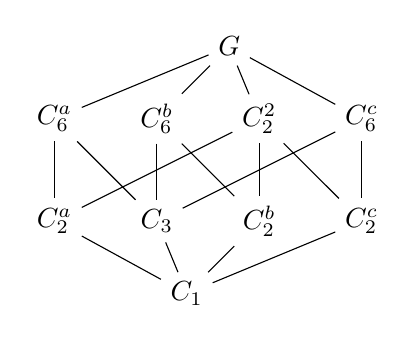
\begin{tikzpicture}[node distance=1.3cm]
        \node(G)[midway]{$G$};
        \node(C6b)[below left of =G]{$C_6^{b}$}; \node(C6a)[left of=C6b]{$C_6^{a}$};  
        \node(C22)[right of=C6b]{$C_2^{2}$};    \node(C6c)[right of=C22]{$C_6^{c}$};
        \node(C2a)[below of=C6a]{$C_2^{a}$};    \node(C3)[below of=C6b]{$C_3$};
        \node(C2b)[below of=C22]{$C_2^{b}$};    \node(C2c)[below of=C6c]{$C_2^{c}$};
        \node(C1)[below left of=C2b]{$C_1$};
        \draw(G)--(C6a);    \draw(G)--(C6b);    \draw(G)--(C6c);    \draw(G)--(C22);
        \draw(C6a)--(C2a);  \draw(C6a)--(C3);
        \draw(C6b)--(C2b);  \draw(C6b)--(C3);
        \draw(C6c)--(C2c);  \draw(C6c)--(C3);
        \draw(C22)--(C2a);  \draw(C22)--(C2b);  \draw(C22)--(C2c);
        \draw(C2a)--(C1);   \draw(C2b)--(C1);   \draw(C2c)--(C1);   \draw(C3)--(C1); 
    \end{tikzpicture}
    \end{figure}
    %There is a Brauer relation coming from the $C_2 \times C_2$-quotient, given by $$\Psi = C_3 - C_6^a - C_6^b - C_6^c + 2G.$$ 
    
    Consider an order $6$ character $\rho_a$ of $G$ with $C_2^{a}$ in its kernel. This has $\bQ(\rho_a) = \bQ(\zeta_6) = \bQ(\sqrt{-3})$. Let $\tau$ generate $\Gal(\bQ(\rho_a) / \bQ)$. One has
    \begin{equation}\label{ex1-rel}\tag{\textdagger}
    \Ind_{C_2^{a}}^G \trivial  \ominus \Ind_{C_6^{a}}^G \trivial \ominus \Ind_{C_2^{2}}^G \trivial \oplus \Ind_G^G \trivial \simeq \rho_a \oplus \rho_a^{\tau} .
    \end{equation}
    Let $E / \bQ$ be a semistable elliptic curve. To apply Theorem \ref{thm_positive_rank}, we need to compute
    \begin{equation}\label{ex1}\tag{*} 
        \frac{C_{E / F^{C_2^a}} C_{E / \bQ} }{C_{E / F^{C_6^a}} C_{E / F^{C_2^2}}} = 
        \frac{C_{E / L} C_{E / \bQ}}{C_{E / L^{C_3}} C_{E / L^{C_2}}}
    \end{equation} 
    where $L = F^{C_2^a}$ has $\Gal(L / \bQ) = C_6$, and check whether it is a norm from $\bQ(\sqrt{-3})$. This is a product of local Tamagawa numbers, as the minimal differential terms are $1$ when $E / \bQ$ is semistable (Lemma \ref{lem_Dterms}(i)). 
    
    One needs to compute these locally for each $p \in \bQ$. If $E / \bQ_p$ has good reduction, then the Tamagawa numbers at all places above $p$ in the subfields of $L$ are $1$. Suppose that $E / \bQ_p$ has split multiplicative reduction at $p$. Let $n = v_p(\Delta_E)$. For $H \leq G$, the Tamagawa number at a prime $\fP$ above $p$ in $L^H$ is given by $c_{\fp}(E / L^H) = e_{\fP \mid p} n$, where $e_{\fP \mid p}$ is the ramification degree. Thus the computation of Tamagawa numbers depends on the choice of decomposition group $D_p \leq C_6$ (to count the number of primes above $p$ in a given subfield) and the choice of inertia group $I_p \leq C_6$ (to compute the ramification indices). 
    
    The following table describes the product of Tamagawa numbers at places above $p$ in our expression, for varying $D_p$ and $I_p$. We let $T_{\fP \mid p}(E / L^H) = \prod_{\fP \mid p}c_{\fP}(E / L^H)$ for $H \leq \Gal(L / \bQ)$ as defined in Notation \ref{not_contr}. Let $C_p = c_p(E / \bQ)T_{\fP \mid p}(E / L) \big/ T_{\fP \mid p}(E / L^{C_3})T_{\fP \mid p}(E / L^{C_2})$. 
    \[
    \begin{array}{c c c c c c c}
        D_p & I_p & c_p(E / \bQ) & T_{\fP \mid p}(E / L^{C_3}) & T_{\fP \mid p}(E / L^{C_2}) & T_{\fP \mid p}(E / L) & C_p\\ 
        \hline
        C_1 & C_1 & n & n^2 & n^3 & n^6 & \square\\
        C_2 & C_1 & n & n & n^3 & n^3 & \square\\
        C_3 & C_1 & n & n^2 & n & n^2 & \square \\
        C_6 & C_1 & n & n & n & n & \square \\
        C_2 & C_2 & n & 2n & n^3 & (2n)^3 & \square \\
        C_6 & C_2 & n & 2n & n & 2n & \square \\
        C_3 & C_3 & n & n^2 & 3n & (3n)^2 & 3\cdot\square \\
        C_6 & C_3 & n & n & 3n & 3n & \square\\
        C_6 & C_6 & n & 2n & 3n & 6n & \square
    \end{array}
    \]

    In all cases we see that $C_p$, the contribution of Tamagawa numbers above $p$, is a norm form $\bQ(\sqrt{-3})$. It is not too hard to check that this is also the case when $E / \bQ_p$ has non-split multiplicative reduction. Therefore the expression in \eqref{ex1} is always a norm from $\bQ(\rho_a)$. This is an example of a more general phenomenon; for cyclic groups we always get a norm. This follows from  Theorem \ref{thm_consistent_cyclic}, which is proven in \S\ref{sec_cyclic}.
    %and $F / \bQ$ an abelian extension with $G = \Gal(F / \bQ)$. We claim that $C(\Theta) \in \fieldnorm{\rho_a}$, for all such $E$. Since each subgroup in $\Theta$ contains $C_2^{a}$, we have that $C(\Theta)$ equals $C(\Theta / C_2^{a})$ where $\Theta / C_2^{a} \in \B(G / C_2^{a}) = \B(C_6)$.  Now $\Theta / C_2^{a}$ is a $\chi_6$-relation, where $\chi_6 = \rho_a^{C_2^a}$ is a faithful order $6$ character of $C_6$, with $\bQ(\chi_6) = \bQ(\rho_a)$. But for cyclic groups we always get norm relations; by Theorem \ref{thm_consistent_cyclic}, $C(\Theta / C_2^{a}) \in \fieldnorm{\rho_a}$.

    But! Observe that{\footnote{this is called a Brauer relation, see Definition \ref{def-brauer}}} 
    \[ \Ind_{C_3}^G \trivial \ominus \Ind_{C_6^a}^G \trivial \ominus \Ind_{C_6^b}^G \trivial \ominus \Ind_{C_6^c}^G \trivial \oplus (\Ind_G^G \trivial)^{\oplus 2} = 0 \]
    as a virtual permutation representation. Append this to the left hand side of \eqref{ex1-rel}. Then Theorem \ref{thm_positive_rank} asks us to compute 
    \begin{equation}\label{ex1-rel2}\tag{**}
    \left(\frac{C_{E / F^{C_2^a}} C_{E / \bQ} }{C_{E / F^{C_6^a}} C_{E / F^{C_2^2}}}\right) \cdot \left( \frac{C_{E / F^{C_3}} C_{E / \bQ}^2}{C_{E / F^{C_6^a}}C_{E / F^{C_6^b}}  C_{E / F^{C_6^c}} } \right). 
    \end{equation}
    
    We can find instances where the second factor is not a norm from $\bQ(\sqrt{-3})$. Indeed suppose $E / \bQ$ has split multiplicative reduction at a prime $p$ with $D_p = G$, $I_p = C_6^b$. Let $v_p(\Delta_E) = n$. Then there is only one prime above $p$ in each subfield. Suppose $E$ has good reduction at all other primes (or multiplicative reduction at primes that are totally split in $F / \bQ$ would also be fine).
     Then our expression \eqref{ex1-rel2} is equal to
     \[ \frac{(6n)(n)}{(2n) (3n)} \cdot \frac{(2n)(n)^2}{(2n)(n)(2n)} \cdot \square = \frac{1}{2} \cdot \square, \] 
     which is not a norm from $\bQ(\sqrt{-3})$. Hence one must have $\rk E / F > 0$. 
\end{example}

\begin{example}[Dihedral]
    Let $q_1, q_2$ be odd primes. Consider $G = D_{2 q_1 q_2}$ the dihedral group of order $2 q_1 q_2$. 
    Let $\rho$, $\tau_1$, $\tau_2$ be two-dimensional irreducible representations of $G$ corresponding to rotating a $(q_1 q_2)$-gon by $2 \pi / q_1 q_2$, $2 \pi / q_1$, $2 \pi/ q_2$ respectively. These are all self-dual. The Galois conjugates of these representations, as well as the trivial $\trivial$ and sign $\epsilon$, yield all the irreducible representations of $G$. Let 
    \[  \sigma_{\rho} = \bigoplus_{ \fg \in \Gal(\bQ(\rho) / \bQ)} \rho^{\fg}, \qquad
        \sigma_1 = \bigoplus_{ \fg \in \Gal(\bQ(\tau_1) / \bQ)} \tau_1^{\fg}, \qquad
        \sigma_2 = \bigoplus_{ \fg \in \Gal(\bQ(\tau_2) / \bQ)} \tau_2^{\fg}. \]  
    Then $ \{ \trivial , \epsilon, \sigma_{\rho}, \sigma_1, \sigma_2 \}$ are a basis for the irreducible representations of $G$ over $\bQ$. 
    One has
\[
        \Ind_{C_2}^G \trivial \simeq \trivial \oplus \sigma_1 \oplus \sigma_2 \oplus \sigma_{\rho}, \quad
        \Ind_{D_{2 q_1}}^G \trivial \simeq \trivial \oplus \sigma_2, \quad
        \Ind_{D_{2 q_2}}^G \trivial \simeq \trivial \oplus \sigma_1,
\]
% There is an irreducible representation $\rho$ of $G$, obtained by inducing a linear order $q_1 q_2$ faithful representation from $C_{q_1 q_2}$. Thus $\rho$ is of degree $2$ and $\bQ(\rho) = \bQ(\zeta_{q_1 q_2})^{C_2}$. Then $\rho$ has $\frac{(q_1 - 1)(q_2 - 1)}{2}$ Galois conjugates, and so $\repnorm{\rho}$ is of dimension $2 \cdot \frac{(q_1 - 1)(q_2 - 1)}{2}$. 
and so 
\begin{equation*}
\Ind_{C_2}^G \trivial \ominus \Ind_{D_{2 q_1}}^G \trivial \ominus \Ind_{D_{2 q_2}}^G \trivial \oplus \Ind_{G}^G \trivial \simeq \bigoplus_{ \fg \in \Gal(\bQ(\rho) / \bQ)} \rho^{\fg}.
\end{equation*}

    Assume $E / \bQ$ is semistable. Suppose that $E / \bQ_p$ has split multiplicative reduction, with $n = v_p(\Delta_E)$. We compute Tamagawa numbers above $p$ as in the previous example, using the same notation. 
    Corollary \ref{cor-odd-decomp} implies that we always get a norm from the contribution above $p$ whenever the decomposition group is a group of odd-order. In fact we only get a non-square contribution when the decomposition group is $D_{2 q_1}$ or $D_{2 q_2}$ (and $I_p$ is non-trivial). 
     
    For example, let $p$ have decomposition group $D_{2 q_1}$ and inertia group $C_{q_1}$.
    This time, counting primes and computing ramification degrees is a little more awkward, we use Exercise \ref{ex-counting}.
        \begin{itemize}[--]
            \setlength\itemsep{0em}
            \item The action of $D_{2 q_1}$ on $C_2 \backslash G$ yields $1$ orbit of size $C_{q_1}$ (the orbit of the identity) and $\frac{q_2 - 1}{2}$ orbits of size $2q_1$ (coming from $C_2$ acting faithfully on $C_{q_2}$). The size of the inertia sub-orbits is $q_1$. Hence $T_{\fP \mid p}(E / F^{C_2}) = (q_1 n)^{1 + \frac{q_2 - 1}{2}}$.
            
            \item The action of $D_{2 q_1}$ on $D_{2 q_1} \backslash G$ yields the same number of orbits as above, but now the action of $C_{q_1} \leq D_{2 q_1}$ is trivial, so that $T_{\fP \mid p}(E / F^{D_{2 q_1}}) = n^{1 + \frac{q_2 - 1}{2}}$.
            
            \item The action of $D_{2 q_1}$ on $D_{2 q_2} \backslash G$ yields one orbit of size $q_1$, with the inertia sub-orbit also of size $q_1$, hence $T_{\fP \mid p}(E / F^{D_{2 q_2}}) = q_1 n$.
        \end{itemize}
    In total,
    \[ \frac{T_{\fP \mid p}(E / F^C_2) \cdot c_{\fp}(E / \bQ)}{T_{\fP \mid p}(E / F^{D_{2 q_1}})\cdot T_{\fP \mid p}(E / F^{D_{2 q_2}})} = \frac{(q_1 n )^{1 + \frac{q_2 - 1}{2}} (n)}{(n)^{1 + \frac{q_2 - 1}{2}} (q_1 n)} = q_1^{\frac{q_2 - 1}{2}} .\] 
    %By symmetry, taking the decomposition group to be $D_{2 q_2}$ and inertia group $C_{q_2}$, one would obtain $ q_2^{\frac{q_1 - 1}{2}}$.

    So let $E / \bQ$ have split multiplicative reduction at $p$ with decomposition group $D_{2 q_1}$ and inertia group $I_p = C_{q_1}$, and good reduction at all other primes. Further suppose that $q_1, q_2 \equiv 3 \pmod 4$ and that $\legendre{q_1}{q_2} = -1$. Then $\bQ(\sqrt{q_1 q_2}) \subset \bQ(\rho)$ but 
$$\frac{C_{E / F^C_2} C_{E / \bQ}}{C_{E / F^{D_{2 q_1}}} C_{E / F^{D_{2 q_2}}}} = q_1 \cdot \square$$
is not a norm from $\bQ(\sqrt{q_1 q_2})$. Indeed, $q_1$ is not the norm of an element of $\bQ(\sqrt{q_1 q_2})$, since $z^2 q_1 = x^2 - q_1q_2 y^2$ for $x,y,z \in \bZ$ implies $q_1 = \square \pmod {q_2}$, a contradiction. Thus $\rk E / F > 0$.

    This rank growth is predicted by root number computations also, however. Assume that $F / \bQ$ is totally real. Then $w(E / F^H) = (-1)^{[F^H \colon \bQ] + | H \backslash G / D_p|}$ by Proposition \ref{compute-root}. Thus
    \begin{itemize}[--]
        \setlength\itemsep{0em}
        \item $w(E / \bQ) = (-1)^2 = 1$,
        \item $w(E / F^{C_2}) = (-1)^{q_1 q_2} (-1)^{1 + \frac{q_2 - 1}{2}} = (-1)^{\frac{q_2 - 1}{2}}$,
        \item $w(E / F^{D_{2 q_1}}) = (-1)^{q_2}(-1)^{1 + \frac{q_2 - 1}{2}} = (-1)^{\frac{q_2 - 1}{2}},$
        \item $w(E / F^{D_{2 q_2}}) = (-1)^{q_1}(-1) = 1$. 
    \end{itemize}
    Therefore we must have $\rk E / F^{C_2}$, $\rk E / F^{D_{2q_1}} > 0$, so $\rk E / F > 0$. 
    Using the properties in Proposition \ref{compute-root-twist}, the computations of the root numbers for the subfields implies that 
    \[ w\left(E / \bQ, \sigma_1\right) = 1, \quad w\left(E / \bQ, \sigma_2\right) = -1, \quad w\left(E / \bQ, \sigma_{\rho}\right) = 1, \]
  and in particular $w(E / \bQ, \tau_1^{\fg}) = -1$ for some $\fg \in \Gal(\bQ(\tau_1) / \bQ)$.
\end{example}

\begin{example}[Additive reduction example]
Let $G = C_{65} \ltimes C_4$, where $C_4$ acts faithfully on $C_{65}$, as well as the subgroups $C_{13}$ and $C_5$. By inducing a faithful character of order $65$ from $C_{65}$, one obtains a faithful irreducible representation $\rho$ of $G$ of dimension $4$ and with $\bQ(\rho) = \bQ(\zeta_{65})^{C_4}$. In particular one has $\bQ(\sqrt{65}) \subset \bQ(\rho)$. Then
\[ \Ind_{C_4}^G \trivial \ominus \Ind_{C_{13} \ltimes C_4}^G \trivial \ominus \Ind_{C_5 \ltimes C_4}^G \trivial \oplus \Ind_{G}^G \trivial \simeq \bigoplus_{\fg \in \Gal(\bQ(\rho) / \bQ)} \rho^{\fg} .\]
Therefore by Theorem \ref{thm_positive_rank}, either 
\begin{equation}\label{ex3}\tag{\textdagger \textdagger}
\frac{C_{E / F^{C_4}} C_{E / \bQ} }{C_{E / F^{C_{13} \ltimes C_4}} C_{E / F^{C_5 \ltimes C_4}}}
\end{equation}
is a norm from $\bQ(\sqrt{65})$, or $\rk E / F > 0$.  

Suppose $p = 5$ and $E / \bQ_p$ has additive, potentially good reduction. Further suppose that $F / \bQ$ is an extension such that $D_{5} = I_{5} = C_5 \ltimes C_4$ (this is wildly ramified). Let $n = v_p(\Delta_E) < 12$. Then
\begin{itemize}[--]
    \setlength\itemsep{0em}
    \item In $F^{C_4}$ there is one prime above $p$ with ramification degree $5$ and $3$ primes above $p$ with ramification degree $20$,
    \item In $F^{C_{13} \ltimes C_4}$ there is one prime above $p$ with ramification degree degree $5$,
    \item In $F^{C_5 \ltimes C_4}$ there is one prime above $p$ with ramification degree $1$ and $3$ primes above $p$ with ramification degree $4$.
\end{itemize}
Therefore, by Lemma \ref{lem_Dterms}(iii), the product of the minimal differential term is 
\[ \frac{D_{\fP \mid p}(E / F^{C_4}) D_{\fP \mid p}(E / \bQ) }{D_{\fP \mid p}(E / F^{C_{13} \ltimes C_4}) D_{\fP \mid p}(E / F^{C_{5} \ltimes C_4})} = 
\frac{ 5^{\floor{5 n /12}} \cdot \left(5^{\floor{20 n /12}}\right)^3 }{5^{\floor{5 n /12}} \left(5^{\floor{4 n /12}}\right)^3} .\]
If $n = 2$, then this is equal to $5 \mod {(\bQ^{\times})^2}$. By Lemma \ref{tamagawa-num} the Tamagawa number product is
\[ \frac{T_{\fP \mid p}(E / F^{C_4}) T_{\fP \mid p}(E / \bQ) }{T_{\fP \mid p}(E / F^{C_{13} \ltimes C_4}) T_{\fP \mid p}(E / F^{C_{5} \ltimes C_4})} = \frac{1^2 \cdot 3^3 }{1^2 \cdot 3^3} = 1 \text{ or } \frac{1^5}{1^5} = 1.\]

We claim that $5$ is not a norm from $\bQ(\sqrt{65})$. Indeed, $5z^2 = x^2 - 65 y^2$ for $x, y, z \in \bZ$ implies that $5 = \square \pmod 13$, a contradiction since $\legendre{5}{13} = \legendre{13}{5} = \legendre{3}{5} = -1$. Therefore the local contribution of \eqref{ex3} above $5$ is not a norm from $\bQ(\sqrt{65})$. 

What are the local root numbers above $p$? By Proposition \ref{compute-root}, one has
\begin{itemize}[--]
    \setlength\itemsep{0em}
    \item $w(E / \bQ_5) = (-1)^{\floor{ 10 / 12}} = 1$, 
    \item $\prod_{\fp \mid p} w(E /F^{C_4}_{\fp}) = (-1)^{\floor{50 / 12}} \left((-1)^{\floor{200 / 12}}\right)^3 = 1$,
    \item $\prod_{\fp \mid p} w(E /F^{C_{13} \times C_4}_{\fp}) = (-1)^{\floor{50 / 12}} = 1$,
    \item $\prod_{\fp \mid p}w(E /F^{C_{5} \times C_4}_{\fp}) = (-1)^{\floor{ 10/12}}\left((-1)^{\floor{40 / 12}}\right)^3 = -1$ .
\end{itemize}
Hence we see a change in the contributions of local root numbers above $p$ in the intermediate subfields. 




\end{example}


\newpage
\section{Forcing points of infinite order}
In [Dok-Wier-Ev], they establish a (dependent on some conjectures) test for forcing a point of infinite order.

\begin{thm}\label{dew-thm}
    Let $E / \bQ$ be an elliptic curve, $F / \bQ$ a Galois extension with Galois group $G$, $\rho$ an irreducible representation of $G$ and 
    \begin{equation}\label{rho-reln}
        \left(\bigoplus_{g \in \Gal(\bQ(\rho) / \bQ)} \rho^g\right)^{\oplus m(\rho)} = 
        \left(\bigoplus_i \Ind_{H_i}^G \trivial \right) \ominus \left(\bigoplus_j \Ind_{H_j'}^G \trivial \right),
    \end{equation}
    for some $m(\rho) \in \bZ$ and subgroups $H_i, H_j' \leq G$. 

    If either $\prod_i C(E / F^{H_i}) / \prod_j  C(E / F^{H_j'})$ is not a norm from some quadratic field $\bQ(\sqrt{D}) \subset \bQ(\rho)$, or if it is not a rational square when $m(\rho)$ is even, then $E$ has a point of infinite order over $F$.
\end{thm}

In this paper, they give two examples of applications of this theorem. Of course, another means of forcing infinite order is via root numbers. We are currently unsure as to whether this norm test is weaker/equivalent/stronger than the test of root numbers. For example, in odd order extensions, root numbers don't tell us anything. We show in the next section that this norm test doesn't either, that is, the product of Tamagawa numbers is always a norm.

\vspace{1em}

As discussed in section \ref{D-loc}, the function on $B(G)$ sending $H \mapsto C(E / F^H)$ is the product of local functions depending on the decomposition group $D_p$ at a prime $p$. We denote each of these as $(D_p, I_p, \psi_p)$, as in definition \ref{D-I-fn}. Then the product of Tamagawa numbers in \ref{dew-thm} is the evaluation of $\prod_p (D_p, I_p, \psi_p)$ on $\sum_i H_i - \sum_j H_j'$.

If we are interested in evaluating each $(D_p, I_p, \psi_p)$ individually, then we have some freedom to change our field extension to make computations easier. In particular, 

\begin{lemma}\label{DeqI}
    In an odd degree unramified extension, Tamagawa numbers change only up to squares. In particular, if $[D_p \colon I_p]$ is odd, then $(D_p, I_p, \psi_p) \sim_{\rho} (D_p, D_p, \psi_p)$ for any $\rho$ with $\bQ(\rho)$ even. 
\end{lemma}

\begin{proof}
    Yadada
\end{proof}


%Let $F_i = F^{H_i}$, $F_j = F^{H_j'}$.
%Note that $$\prod_i C(E / F_i) / \prod_j  C(E / F_j')  = \prod_p \left(\prod_i  C_{p}(E / F_i) /  \prod_j C_{p}(E / F_j')\right)$$
%where $C_p(E / F_i) =\prod_{v | p} c_v(E / F_i)\cdot |\omega / \omega_{v, \min}|$.

%Let $D_p$, $I_p$ be the decomposition and inertia subgroups of $G$ at $p$.
%The function on the Burnside ring of $G$ sending $H$ to $C_p(E / F^H)$ is then of the form $(D_p, I_p, \psi_p).$ 


\subsection{Norm relations in odd order extensions}

{\color{red} add some motivation (justification) for why I'm proving this result. The point is that the test for positive rank provided by root number computations never says anything in odd order extensions. If we expect the norm relations test to be weaker than root numbers, then nor should this test.}

\begin{thm}\label{odd-exts}
 Let $E / \bQ$ be an elliptic curve, $F / \bQ$ be an extension of \textbf{odd order} with Galois group $G$. 
 
Suppose that the primes of additive reduction of $E$ are at worst tamely ramified in $F / \bQ$ (and $\geq 5$). 
Take any representation $\rho \in R(G)$ with quadratic subfield $\bQ(\sqrt{D}) \subset \bQ(\rho)$ and relation
\begin{equation*}\label{odd-exp}
 \left(\bigoplus_{\mathfrak{g}\in\Gal(\QQ(\rho)/\QQ)}\rho^{\mathfrak{g}}\right)^m=\bigoplus_i\Ind_{F_i/\QQ}\mathds{1}\ominus\bigoplus_j\Ind_{F'_j/\QQ}\mathds{1}
\end{equation*}
 as in theorem \ref{thm_positive_rank}. Then
 \[ \frac{\prod_i C_{E/F_i}}{\prod_j C_{E/F_j'}}  \in 
    \begin{cases}
        N_{\bQ(\sqrt{D}) / \bQ}(\bQ(\sqrt{D})^{\times}) & m \ \text{odd}, \\
        \bQ^{\times 2} & m \ \text{even}.
    \end{cases} \] 
    In other words, one cannot use theorem \ref{thm_positive_rank} to conclude that $E / F$ must have positive rank. 
\end{thm}
Let us break up the function $C \colon H \mapsto C_{E / F^H}$ into $C = \prod_p  \fc_p \cdot d_p$ where
\begin{equation}\label{c-and-d}
         \fc_p(H) = \prod_{v | p}  c_v(E / F^H) , \qquad d_p(H) = \prod_{v | p} \left|\frac{\omega}{\omega_{v}^{\min}}\right|_v, 
\end{equation}
the product ranging over all finite places of $F^H$ dividing $p$.
Then $\fc_p$ and $d_p$ are $D_p$-local functions. Let $D_p = \Gal(F_w / \bQ_p)$, where $F_w$ denotes the completion of $F$ with respect to a place $w$ lying above $p$. Recall the notation that for a number field $K$ and place $v$, $C_v(E / K) = c_v(E / K) \cdot \left| \omega / \omega_v^{\min} \right|_v.$ 
Then
\begin{equation}\label{Dp-loc}
\fc_p \cdot d_p = (D_p, f_p)
\end{equation}
where $f_p$ is a function on $B(D_p)$ with $H \mapsto C_v(E / F_w^H)$.
%We will observe throughout that if $v$ is a place of $F^H$ corresponding to the double coset $HxD_{p}$, then $C_v(E / F^H)$ is a function of $e_v$ and $f_v$. Thus we have
%\[ \fc_p \cdot d_p = (D_p, I_p, C_v) \]

We first argue that it is enough to prove this theorem when $m$ is the order of $\repnorm{\rho}$ in $C(G)$. 

\begin{lemma}
    Consider the set-up as in theorem \ref{odd-exts}. If the statement of the theorem holds when $m$ is the order of $\repnorm{\rho}$ in $C(G)$, then it holds for all possible $m$. {\color{red} really, this is saying that if $f$ is trivial on Brauer relations, then showing it is trivial on rho-relations for minimum m is enough (maybe I could add that in rep theory section)}
\end{lemma}

\begin{proof}
    By definition, if $m$ is the order of $\repnorm{\rho}$ in $C(G)$ then there exists $\Theta \in B(G)$ such that $\bC[\Theta] \simeq \repnorm{\rho}^{\oplus m}$.
    Now consider $n$ and $\Psi \in B(G)$ such that $\bC[\Psi] \simeq \repnorm{\rho}^{\oplus n}$. Clearly $m \mid n$.  Then $\Phi = \Psi - \frac{n}{m}\Theta$ is a Brauer relation.

    At this point, we use that the function $C$ on $B(G)$, viewed as a function to $\bQ^{\times} / \bQ^{\times 2}$, is trivial on Brauer relations. For odd order groups this follows from \cite[Theorem 2.47]{reg-const} and \cite[Theorem 3.2  (Tam)]{reg-const}, looking locally at each $C_p$. 
    Then $C(\Psi) = C(\Theta)^{n / m} \cdot C(\Phi)$ so $C(\Psi) \equiv C(\Theta)^{n / m} \mod \bQ^{\times 2}$. It follows that if $C(\Theta)$ satisfies the conditions of theorem \ref{odd-exts}, then so does $C(\Psi)$.
\end{proof}

Taking $m$ to be the order of $\repnorm{\rho}$ in $C(G)$, we have that $m$ divides $|G|$, hence is odd. Therefore we need to prove that, given any $
\Theta \in B(G)$ such that $\bC[\Theta] \simeq \repnorm{\rho}^{\oplus m}$, the expression $C(\Theta)$ is the norm of an element from $\bQ(\sqrt{D})^{\times}$.
Replacing $\rho$ by the sum of its conjugates by elements of $ \Gal(\bQ(\rho) / \bQ(\sqrt{D}))$, we may assume that $\bQ(\rho) = \bQ(\sqrt{D})$. Note that this does not affect $m$. 

We record
\begin{table}[H]
         \vspace{-1em}
         \setlength\itemsep{0em}
        \centering
\begin{tabular}{l l}
    $\tau$ & the generator of $\Gal(\bQ(\sqrt{D}) / \bQ)$, \\
    $k$ & the smallest integer such that $\bQ(\sqrt{D}) \subset \bQ(\zeta_k)$. Then $k \mid |G|$, hence is odd.
\end{tabular}
\vspace{-1em}
\end{table}
Fix $\Theta = \sum_i n_i H_i \in B(G)$ with $\bC[\Theta] \simeq \repnorm{\rho}^{\oplus m}$. We prove that at each prime $p$, $\fc_p(\Theta)$ and $d_p(\Theta)$ are the norms of elements from $\bQ(\rho)^{\times}$.  These depends on $D_p$ and $I_p$ ; the decomposition and inertia group respectively at $p$. As we deal with each local factor individually, we argue that one can take $D_p = I_p$.

\begin{lemma}\label{tam-up-to-square}
    Let $E / K$ be an elliptic curve. Let $K' / K$ be an extension of number fields odd degree, unramified at the place $v$ of $K$. Then $C_w(E / K') \equiv C_v(E / K) \mod \bQ^{\times 2}$ for any place $w$ of $K'$ with $ w \mid v$. 
\end{lemma}

\begin{proof}
This is automatic for good reduction and split multiplicative reduction. It is also clear for non-split multiplicative reduction since the residue degree cannot be even (so the reduction type remains non-split at $w$). For additive reduction, see \cite[Lemma 3.12]{reg-const}.
\end{proof}

\begin{lemma}\label{DeqI}
    At a prime $p$, we may assume that $D_p = I_p$ when computing $(\fc_p \cdot d_p)(\Theta)$. 
\end{lemma}

\begin{proof}
Let $p$ have residue degree $f_p$. Let $L / \bQ$ be a Galois extension of degree $f_p$ with cyclic Galois group, such that $p$ is inert in $L$. Further ensure that $F \cap L = \bQ$. Then $\Gal(FL / L) = G$. Let $F_i = F^{H_i}$ and $L_i = F_i L$.

Let $v$ be a place over $p$ in $F_i$. The extension $L_i / F_i$ is Galois, so $v$ is either split or inert in $L_i$.
We claim that $C_v(E / F_i) \equiv \prod_{w | v} C_w(E / L_i) \mod \bQ^{\times 2}$. Indeed, the number of terms in the product on the right is odd, and by lemma \ref{tam-up-to-square} $C_v(E / F_i) \equiv C_w(E / L_i) \mod \bQ^{\times 2}$. 
Letting $\fc_p'$ and $d_p'$ be functions on $B(G)$ defined as in (\ref{c-and-d}) but with $\bQ$, $F$ replaced by $L$, $FL$, we see that $(\fc_p \cdot d_p)(\Theta) \equiv (\fc_p' \cdot d_p')(\Theta) \mod \bQ^{\times 2}$. 
Thus it is equivalent to do our computation in $FL / L$, but here $p$ has residue degree $1$.
\end{proof}

We also show that if $\bQ(\Res_{D_p} \rho) = \bQ$, then $(\fc_p \cdot d_p)(\Theta) \in \bQ^{\times 2}$.

\begin{lemma}\label{rational-res}
    Let the exponent of $D_p$ be $b$. If $k \nmid b$, then $(\fc_p \cdot d_p)(\Theta) \in \bQ^{\times 2}$. 
\end{lemma}

\begin{proof}
    Note that $\bQ(\Res_{D_p}{\rho}) \subset \bQ(\zeta_b) \cap \bQ(\rho) \subset \bQ(\zeta_b)$. Then $\bQ(\rho) \subset \bQ(\zeta_b) \implies k \mid b$ by minimality of $k$. Since $k \nmid b$, we have $\bQ(\rho) \not\subset \bQ(\zeta_b)$, so $\bQ(\Res_{D_p} \rho) = \bQ$ and $\Res_{D_p} \rho = \tau (\Res_{D_p} \rho)$. 
    
    Now $\bC[\Res_{D_p} \Theta] \simeq (\Res_{D_p} \rho)^{\oplus 2 m} \in \Perm(D_p)$. Since $C(D_p) = \Char_{\bQ}(D_p) / \Perm(D_p)$ has odd order, it follows that $(\Res_{D_p} \rho)^{\oplus m} \in \Perm(D_p)$.  
    Therefore there is $\Theta' \in B(D_p)$ such that $\bC[\Theta'] \simeq (\Res_{D_p} \rho)^{\oplus m}$. Then $\Psi = (\Res_{D_p}\Theta) - 2 \Theta'$ is a Brauer relation for $D_p$. Then 
    \[(\fc_p \cdot d_p)(\Theta) \ {\ov{(\ref{Dp-loc})}{=}} \ f_p(\Res_{D_p}\Theta)
    = f_p(\Psi) \cdot f_p(\Theta')^2 \in \bQ^{\times 2}. \]
    Again we are using \cite[Theorem 2.47]{reg-const} and \cite[Theorem 3.2]{reg-const} which imply that $f_p(\Psi) \in \bQ^{\times 2}$ when $\Psi$ is a Brauer relation for $D_p$ (since $D_p$ is odd).   
\end{proof}


To prove theorem \ref{odd-exts}, we proceed by considering separately each reduction type.

\subsubsection*{Good reduction}
If $E / \bQ$ has good reduction at $p$,it has good reduction at all primes lying above $p$ in subfields of $F$. Hence the Tamagawa number is always one, as well as $\left|\omega / \omega_{v}^{\min}\right|_v$ for any place $v \mid p$ in an intermediate field. Therefore $\fc_p$, $d_p = 1$ as functions on $B(G)$.

\subsubsection*{Multiplicative reduction}

If $E / \bQ_p$ has multiplicative reduction, then as in the good reduction case one has $\left|\omega / \omega_{v}^{\min}\right|_v = 1$ for any place $v \mid p$ in an intermediate field. Thus $d_p = 1$.
For $\fc_p$, we consider non-split/split reduction separately.
\vspace{1em}

\noindent\underline{\textit{Non-split multiplicative reduction}}

Let $E / \bQ_p$ have non-split multiplicative reduction. Since $D_p = I_p$, all primes above $p$ have residue degree $1$. Then the reduction at places above $p$ remains non-split in all intermediate subfields.
It follows that 
\[ \fc_p = (D_p, \alpha) \]
where $\alpha$ is the constant function on $B(D_p)$ with $\alpha \in \{1, 2\}$, depending on $\ord_p(\Delta)$ being even or odd. 
We prove a more general lemma that $D_p$-local constant functions are trivial on $\rho$-relations.

\begin{lemma}\label{const-fns}
Let $G$, $\rho$ be as above. The function $(D_p, \alpha)$ for $\alpha \in \bQ^{\times}$ satisfies $(D_p, \alpha)(\Theta) \in \bQ^{\times 2}$.  
\end{lemma}   

\begin{proof}
    The function $(D_p, \alpha)$ on $B(G)$ sends $H \leq G$ to $\alpha^{| H \backslash G / D_p|}$. Thus if $\Theta = \sum_i n_i H_i$ is a $\rho$-relation, $(D_p, \alpha)(\Theta) = \alpha^{ \sum_i n_i \cdot | H_i \backslash G / D_p|}$. We show that $\sum_i n_i \cdot | H_i \backslash G / D_p|$ is even. 

    %Since $G$ is odd, each $| H_i \backslash G / D_p|$ is odd. On the other hand, $\rho \oplus \tau(\rho)$ has even dimension. Therefore $\sum_i |n_i|$ is even. 
    One has $\Res_{D_p} \Theta = \sum_i n_i \sum_{x \in H_i \backslash G / D_p} D_p \cap H^{x^{-1}}$ and the permutation representation $\bC[\Res_{D_p} \Theta]$ of $D_p$ is isomorphic to $\Res_{D_p} (\rho^{\oplus m} \oplus \tau(\rho^{\oplus m}))$. In particular the dimension is even. The dimension is $$\sum_i n_i \sum_{x \in H_i \backslash G / D_p} [D_p \colon D_p \cap H^{x^{-1}} ].$$ Since each $[D_p \colon D_p \cap H^{x^{-1}} ]$ is odd, this implies there are an even number of terms in the summation, i.e. that $\sum_i n_i \cdot | H_i \backslash G / D_p|$ is even. 
    
\end{proof}

\noindent\underline{\textit{Split multiplicative reduction}}

Now suppose $E / \bQ_p$ has split multiplicative reduction. The reduction type remains split at all places above $p$ within sub-extensions of $F / \bQ$. Let $\ord_p(\Delta) = n$. Then 
\[ \fc_p = (D_p, D_p, en). \]
Since the $n$ factor is constant, $(D_p, D_p, en)(\Theta) \equiv (D_p, D_p, e)(\Theta) \mod \bQ^{\times 2}$ by lemma \ref{const-fns} .

We have $D_p = I_p = P_p \ltimes C_l$, where $P_p \triangleleft I_p$ is wild inertia, and $C_l = I_p / P_p$ is the tame quotient. $C_l$ is a cyclic group, with $l \mid p^f - 1 = p - 1$. By lemma \ref{rational-res}, it is only of interest to consider such $D_p$ with exponent  $p^u l$ for some $u \geq 0$ such that $k \mid p^u l$.

Now, $(D_p, D_p, e)(\Theta)$ is the product of ramification indices at primes above $p$. We separate the $p$-part and tame part of this expression.
Recall that the ramification index of a place $w$ above $p$ corresponding to the double coset $H_i x D_p$ has ramification degree $e_w = \frac{|I_p|}{|H_i \cap I_p^x|} =\frac{|I_p|}{|I_p \cap H^{x^{-1}}|}$.
This is the dimension of the permutation representation $\bC[D_p / D_p \cap H^{x^{-1}}]$.
Let  $D_p \cap H^{x^{-1}} = P' \ltimes C_a$ where $P' \leq P$ and $a | l$. Then the ramification index is $\frac{|P|}{|P'|}\cdot \frac{l}{a}$. 

Taking fixed points under wild inertia, one has $$\bC[D_p / D_p \cap H^{x^{-1}}]^{P_p} \simeq \bC[D_p / P_p (D_p \cap H^{x^{-1}})] \simeq \bC[D_p / P_p \ltimes C_a].$$ This permutation representation has dimension $\frac{l}{a}$, so we've killed off the $p$-part. 
Then $$\bC[\Res_{D_p} \Theta]^{P_p} \simeq \left(\Res_{D_p} \rho^{\oplus m} \oplus \tau\left(\Res_{D_p}\rho^{\oplus m}\right)\right)^{P_p},$$
and we can consider these as representations of $D_p / P_p = C_l$.

Let $\Psi = P_p \cdot \Res_{D_p}\Theta / P_p \in B(C_l)$.
Consider the function $g$ on $B(C_l)$ with $H \mapsto [C_l \colon H] = \dim \bC[C_l / H]$. 
It follows from the above discussion that $(D_p, D_p, e)(\Theta)$ differs from $g(\Psi)$ up to a factor of $p$. 

%$(C_l, C_l, e)$ evaluated at $P_p \cdot \Res_{D_p}\Theta / P_p$ equals $(D_p, D_p, \psi_p)$ evaluated at $\Res_{D_p} \Theta$ modulo squares up to (possibly) a factor of $p$.

Crucially, this factor of $p$ doesn't matter:

\begin{lemma}
    Let $K = \bQ(\sqrt{D})$ be a quadratic field, contained in the minimal cyclotomic field $\bQ(\zeta_k)$ with $k$ odd. Let $k \mid p^u l $, for some $u \geq 0$ and $l$ such that $p \equiv 1 \pmod l$. Then $p$ is the norm of an element from $K^{\times}$.
\end{lemma}

\begin{proof}
    Since $k$ is odd, it is clear that $D = \prod_{q | k} q^*$, the product being taken over primes dividing $k$. Note that if $q \not= p$, then since $q \mid l$, we have $p \equiv 1 \pmod l \implies p \equiv 1 \pmod q$. By theorem \ref{p-one-mod-disc},  $p$ is the norm of a principal fractional ideal of $K$. If $K$ is imaginary, then $p$ is the norm of an element of $K$. Else, we invoke theorem \ref{p-norm-elem-1} or theorem \ref{p-norm-elem-2}.
    %We show that $p$ has residue degree $1$ in the extended genus field $E^{+} = K(\{\sqrt{q^*} \colon q | k \})$ of $K$ ({\color{red} cf. appendix}).
    %If $q \not= p$ then $q \mid l$, so $p \equiv 1 \pmod l$. Therefore $p$ splits in any quadratic subfield of $E^{+}$ of discriminant not divisible by $p$. Else, $p$ ramifies in any quadratic subfield with discriminant divisible by $p$. Thus it is clear that $p$ has residue degree $1$ in $E^{+}$, hence also in the genus field $E$, and it follows from theorem \ref{p-principal} that $p$ is the norm of a principal ideal.  Else, we invoke theorem \ref{minus-one-norm}.
\end{proof}

Therefore we only need to worry about the tame part of our ramification indices. If $k \nmid l$, then $\phi = (\Res_{D_p} \rho)^{P_p}$ (viewed as a representation on $D_p / P_p$) has rational character. Then, arguing as in lemma \ref{rational-res}, $g(\Psi) \in \bQ^{\times 2}$ {\color{red} say more?}.
Hence we may assume that $k \mid l$ and that $\bQ(\phi) = \bQ(\rho) = K$.

\begin{prop}\label{semi-stable-gd}
    Let $k \mid l$. Then $g(P_p \cdot \Res_{D_p}\Theta / P_p) = g(\Psi) \in N_{K / \bQ}(K^{\times})$.   
\end{prop}

\begin{proof}
    Write $\phi^{\oplus m} \oplus \tau(\phi^{\oplus m}) = \bC[\Psi] = \sum_{l' \mid l}{a_{l'}} \chi_{l'}$ where $a_{l'} \in \bZ$ and $\chi_{l'}$ are defined in example \ref{cyclic-relns}. Let $\Psi_{l'} = \sum_{l'' | l'}\mu(l' / l'')\cdot C_{l / l''}$ so that $\bC[\Psi_{l'}] = \chi_{l'}$, as observed in the example. Then $\bC[\Psi] \simeq \bC[\sum_{l' | l } a_{l'} \Psi_{l'}]$ which implies that $\Psi = \sum_{l' | l } a_{l'} \Psi_{l'}$ since cyclic groups have no Brauer relations.

    Evaluating $g$ on $\Psi_{l'}$ is trivial unless $l' = q^a$ for some $q$ prime, $a \geq 1$. Indeed, if $l' = p_1^{e_1} \cdots p_r^{e_r}$ , with $r \geq 2$ and $e_i \geq 1$, then
    \[ \prod_{l'' \mid l'} (l'')^{\mu(l' / l'')} = \prod_{j_1, \ldots j_r \in \{0,1\}^r } \left(p_1^{e_1 - j_1} \cdots p_r^{e_r - j_r}\right)^{\# j_i = 1} = \prod_{i = 1}^r \left(\frac{p_i^{e_i}}{p_i^{e_i - 1}}\right)^{\sum_{ j = 0}^{r - 1} \binom{r-1}{j} (-1)^j} = 1. \]
    On the other hand,
    \[ \prod_{l' \mid q^a} (l')^{\mu(q^a / l')} = q .\]
    
    We claim that $k \nmid l'$ implies $a_{l'}$ is even. The irreducible representations of $C_l$ over $\bQ(\phi)$ are given by the orbits of the complex irreducible characters of $C_l$ acted upon by $H = \Gal (\bQ(\zeta_l) / \bQ(\phi))$. One has $\chi_{l'} = \repnorm{\varphi_{l'}}$ where $\bQ(\varphi_{l'}) = \bQ(\zeta_{l'})$. If $ k \nmid l'$ then $\bQ(\phi) \not\subset \bQ(\zeta_{l'})$, so that $B = \Gal(\bQ(\zeta_l) / \bQ(\zeta_{l'})) \not\leq H$. Then $\bQ(\phi) \cap \bQ(\zeta_{l'}) = \bQ$ so $BH = \Gal(\bQ(\zeta_l) / \bQ)$. The orbit of $\varphi_{l'}$ under $H$ is fixed by $BH$, hence is rational. It follows that $\langle \phi, \varphi_{l'} \rangle = \langle \tau(\phi) , \varphi_{l'} \rangle$ so that $a_{l'}$ is even.  

    Thus we can only possibly get something interesting if $k = q$ is a prime. But then $q$ is a norm from $\bQ(\sqrt{q^*})$ by corollary \ref{p-principal}. 
\end{proof}

\subsubsection*{Additive reduction}

Now suppose that $E / \bQ_p$ has additive reduction. In this case, assume that $p \geq 5$. We have $D_p = P_p \ltimes C_l$ with $ l \mid p - 1$.  
%is at worst tamely ramified in $F / \bQ$. This ensures that $D_p = I_p = C_l$ is cyclic, and $l \mid p - 1$. 
Once again we may assume that $k \mid p^k l$ where $p^k l $ is the exponent of $D_p$ by lemma \ref{rational-res}.

Let $\delta = \ord_p(\Delta_E)$. Consider a place $w$ of $F^H$ over $p$ with ramification degree  $e_w$over $\bQ$. Then $\Delta_E$ has valuation $n e_w$ with respect to $w$. Then $\left| \Delta_E / \Delta_{E, w}^{\min} \right|_w = p^{-(\delta\cdot e_w - \delta_H)}$, where $\delta_H = \ord_w(\Delta_{E, w}^{\min})$.
Recall that
\[ \left| \frac{\omega}{\omega_{w}^{\min}} \right|_{w}^{-12} = \left| \frac{\Delta_E}{\Delta_{E, w}^{\min}} \right|_w .\] 
Therefore $\left| \omega / \omega_{w}^{\min} \right|_w = p^{\floor{\frac{\delta\cdot e_w - \delta_H}{12}}}$.

Suppose that $E / \bQ_p$ has Kodaira type $I_n^*$, so $\delta = 6 + n$. For a finite extension $K' / \bQ_p$ with ramification degree $e$, $E / K'$ has Kodaira type $I_{en}^*$ if $e$ is odd, and type $I_{en}$ if $n$ is even. Thus in odd degree extensions the reduction type will stay potentially multiplicative. Then $\delta \cdot e_w - \delta_H = 6 e_w$.

If $E / \bQ_p$ has potentially good reduction then $\delta \in \{2,3,4,6,8,9,10 \}$. $E$ also has potentially good reduction at the place $w$ in $F^H$. Hence $\delta_H \leq 12$ and it follows that $\delta_H = \delta \cdot e_w - 12 \cdot \floor{\delta \cdot e_w /12}$.

In conclusion, 
\[ d_p = 
    \begin{cases}
        (D_p, D_p,\ p^{\floor{e_w /2}}) & \text{if } E \text{ has potentially multiplicative reduction}, \\
        (D_p, D_p,\ p^{\floor{\delta \cdot e_w/12}}) & \text{if } E \text { has potentially good reduction}.
    \end{cases}
    \]

In either case, $d_p(\Theta) \in N_{\bQ(\rho) / \bQ}(\bQ(\rho)^{\times})$. Indeed, this takes values $1$ or $p$ in $\bQ^{\times} / \bQ^{\times 2}$. But $p \equiv 1 \pmod l$ implies $p \equiv 1 \pmod k$ so that $p$ is the norm of a principal ideal in $\bQ(\rho)$, and hence the norm of an element, by corollary \ref{p-one-mod-disc} and theorem \ref{p-norm-elem-1}.

%\[ \left|\frac{\Delta_{E}}{\Delta_{E, w}^\min} \right|_w = p^{f_w 12 \cdot \floor{e_w n / 12}} \implies 
%       \left|\frac{\omega}{\omega_{w}^\min} \right|_w = p \]

For the Tamagawa number computations we use the following description from \cite{reg-const}.

\begin{lemma}[{\cite[Lemma 3.22]{reg-const}}]\label{tamagawa-num}
    Let $L' /L / \bQ_p$ be finite extensions and $p \geq 5$. Let $E / L$ be an elliptic curve with additive reduction; 
    \[ E \colon y^2 = x^3 + Ax + B, \qquad A, B \in L \]
    with discriminant $\Delta = -16(4 A^3 + 27 B^2)$. Let $\delta = v_L(\Delta)$, and $e = e_{L' / L}$.

    If $E$ has potentially good reduction, then 
        \[
        \begin{array}{l l l l}
            \gcd(\delta e, 12) = 2 & \implies & c_v(E / L') = 1, & \quad (II, II^*) \\
            \gcd(\delta e, 12) = 3 & \implies & c_v(E / L') = 2, & \quad (III, III^*) \\
            \gcd(\delta e, 12) = 4 & \implies & c_v(E / L') = \begin{cases} 1, & \sqrt{B} \notin L'
                                \\ 3, & \sqrt{B} \in L' \end{cases}, & \quad (IV, IV^*) \\
            \gcd(\delta e, 12) = 6 & \implies & c_v(E / L') = \begin{cases} 2, & \sqrt{\Delta} \notin L'
                \\ 1 \ \text{or} \ 4, & \sqrt{\Delta} \in L' \end{cases}, & \quad (I_0^*) \\
            \gcd(\delta e, 12) = 12 & \implies & c_v(E / L') = 1. & \quad (I_0)
        \end{array}
        \]

    If $E$ has potentially multiplicative reduction of type $I_n^*$ over $L$, and $e$ is odd, then it has Kodaira type $I_{en}^*$ over $L'$. Moreover, 
    \[
        \begin{array}{l l l l}
        2 \nmid n & \implies & c_v(E / L') = \begin{cases} 2, & \sqrt{B} \not\in L', \\ 4, & \sqrt{B} \in L'. \end{cases} & \quad (I_{ne^*}) \\
        2 \mid n & \implies & c_v(E / L') = \begin{cases} 2 & \sqrt{\Delta} \not\in L', \\ 4 & \sqrt{\Delta} \in L' .\end{cases} & \quad ({I_{ne}^*})   
        \end{array} 
    \]
\end{lemma}

\vspace{2em}

Firstly suppose that $E / \bQ_p$ has reduction type $I_{n}^{*}$. 
Write $D_p = \Gal(F_w / \bQ_p)$. Since we assume $D_p = I_p$, i.e. the residue degree is one, it follows that any subextension $L'$ of $F_{w} / \bQ_p$ satisfies $\sqrt{B} \in L' \iff \sqrt{B} \in \bQ_p$ and $\sqrt{\Delta} \in L' \iff \sqrt{B} \in \bQ_p$. 
Therefore $c_p = (D_p, \alpha)$ where $\alpha \in \{2, 4\}$. But then $(D_p, \alpha)(\Theta) \in \bQ^{\times 2}$ by lemma \ref{const-fns}.\\

Now suppose that $E / \bQ_p$ has potentially good reduction. Observe that in a totally ramified extension of degree coprime to $12$, the Tamagawa number remains the same. Hence for $D_p$ odd, if $3 \nmid |D_p|$ it follows that $c_p = (D_p, \alpha)$ for some constant $
\alpha$ and so $c_p(\Theta) \in \bQ^{\times 2}$.

Thus we assume that $3 \mid |D_p|$. Since we assumed $p \geq 5$, we have $D_p = I_p = P_p \ltimes C_l$ with $3 \mid l$ and $p \equiv 1 \pmod l$. 
If we have type $III$ or $III^*$ or $I_0^*$ then the Tamagawa number is still unchanged in any totally ramified extension of odd degree extension, even when the degree is divisible by $3$. We will treat the other cases separately: 

\vspace{1em}

\noindent\underline{\textit{Type $II$ and $II^*$ reduction:}}

Suppose $\delta = 2$, that is we have Type $II$ reduction. If $L' / \bQ_p$ is an odd degree extension that is divisible by $3$, then $E / L'$ has reduction type $I_0^*$. By by lemma \ref{tamagawa-num} the Tamagawa number of $E / L'$ then depends on whether $\sqrt{\Delta} \in \bQ_p$. Since we have additive reduction, we know that $p \mid A$, $p \mid B$. Moreover, $\delta = 2$ implies that $v_p(B) = 1$. Then, $\Delta = p^2\cdot \alpha$, and $\alpha \equiv -27\cdot\square \pmod p$. Therefore $\sqrt{\Delta} \in \bQ_p \iff -3$ is a square $\pmod p$. But this is the case; we assumed $p \equiv 1 \pmod l$, so $p \equiv 1 \pmod 3$. Then $\legendre{-3}{p} = \legendre{p}{3} = 1$. Therefore the Tamagawa number will be $1$ or $4$, which is a square.
On the other hand if $L' / \bQ_p$ is an extension of odd degree then the reduction type over $L'$ is $II$ or $II^*$ and the Tamagawa number is $1$. It follows that $c_p(\Theta)$ is a product of square terms, so is itself square. 

If $\delta = 10$, then $E / L'$ has reduction type $I_0^*$ whenever $3 \mid [ L' \colon \bQ_p]$. Once more, $v_p(A)$, $v_p(B) \geq 1$, and $v_p(\Delta) = 10 = \min(3 v_p(A), 2 v_p(B)) \implies v_p(B) = 5$. Therefore we get $\Delta = p^{10} \cdot \alpha$ with $\alpha \equiv -27\cdot\square \pmod p$, and we conclude as above.

\vspace{1em}

\noindent\underline{\textit{Type $IV$ and $IV^*$ reduction:}}

Now, if $E /\bQ_p$ has additive reduction of type $IV$ or $IV^*$, it attains good reduction over any totally ramified cyclic extension of degree divisible by $3$. This could result with $3$ coming up an odd number of times in $c_p(\Theta)$, when $\sqrt{B} \not\in \bQ_p$. 
%We show that for both types, one has $\sqrt{B} \in \bQ_p$. 
%Indeed, if $\delta = 4$, then $v_p(B) = 2$, and $v_p(A) \geq 2$. 
%\vspace{1em}
%In summary, 
%\begin{equation}
 %   \prod_{d ' \mid d} C(E / F_{\fp}^{D_{d'}})^{\mu(d / d')}
  %  = 
   % \begin{cases}
    %    1 & 3 \nmid d, \\
    %   1 & 3 \mid d, \delta \in \{0, 3, 6, 9\}, \\
    %    1 \cdot \square & 3 \mid d, \delta \in \{2, 10\}, \\
    %    3^a \cdot\square, a \in \{0,1\} & 3 \mid d, \delta \in \{4,8\}.
    %\end{cases}
%\end{equation}
\begin{rem}
   There's no reason why we can't get 3; see elliptic curve 441b1 with additive reduction at $7$ of type IV and Tamagawa number equal to $3$
\end{rem}

\textbf{If $D_p = C_l$ then we are able to finish our argument.} As in the proof of proposition \ref{semi-stable-gd}, there exists $a_{l'} \in \bZ$ such that $\Res_{D_p}\Theta = \sum_{l' \mid l} a_{l'} \Psi_{l'}$ where $\Psi_{l'} \in B(G)$ is such that $\bC[\Psi_{l'}] \simeq \chi_{l'}$, as in example \ref{cyclic-relns}.

Recall from the proof of lemma \ref{const-fns} that $\Res_{D_p} \Theta = \sum_i n_i \sum_{x \in H_i \backslash G / D_p} D_p \cap H^{x^{-1}}$, with $\sum_i n_i | H_i \ G / D_p|$ even. If $D_p = \Gal(F_w / \bQ_p)$, then the number of subextensions divisible by $3$ (i.e. the number of subextensions where we obtain good reduction ) corresponds to the number of subgroups with index divisible by $3$ in $\Res_{D_p}\Theta$. We compute this number to determine $\ord_3(c_p(\Theta))$ modulo squares.

Let $\psi$ be an irreducible character of $D_p$ of order $3$. We have 
\[ \langle \Ind_{C_{l / l'}}^{C_l} \trivial , \psi_3 \rangle = \begin{cases} 1 & 3 \mid l' \\ 0 & 3 \nmid l'. \end{cases}\] 

Therefore computing $\langle \Res_{D_p} \Theta, \psi_3 \rangle$ will give us the number of subgroups in our expression of index divisble by $3$. Observe that $\langle \chi_{l'}, \psi_3 \rangle = 0$ unless $l' = 3$, in which case it is $1$. Therefore 
\[ c_p(\Theta)  \equiv 3^{a_3} \mod \bQ^{\times 2} \]

As in the proof of \ref{semi-stable-gd}, we observe that $a_3$ is even unless $k \mid 3$,  i.e. that $\bQ(\rho) = \bQ(\sqrt{-3})$. But then $3$ is a norm in $\bQ(\rho)$. Thus we see that in all cases $c_p(\Theta) \in N_{\bQ(\rho) / \bQ}(\bQ(\rho)^{\times})$. 

{\color{red} but probably because the 3 divisibility is in the tame part I could do the whole take $P_p$ fixed points and then pass to $D_p / P_p$ and do the counting there??? hmmm }

%However, it turns out we will only get $3$ occurring oddly when $d = 3$. Indeed, one has that $\langle \Ind_{D_{d'}}^D \trivial, \psi_3 \rangle = 1$ if $3 \mid d'$, and $0$ if $3 \nmid d'$, where $\psi_3$ is an irreducible character of $D$ of order $3$. Therefore one sees that the number of places with ramification degree divisible by $3$ cancels unless $d = 3$. Indeed, $\langle \chi_d , \psi_3 \rangle = 0$ unless $d = 3$, 
%in which case it is $1$. Therefore (\ref{tam-contrib}) can only be non-square when $d = 3$. {\color{red} then conclude why this is fine}

%\begin{lemma}
%    Consider $M / L$ a field extension. Let $E / L$ be an elliptic curve, $v$ a finite place of $L$ and $w$ a finite place of $M$ with $w \mid v$. Let $\omega_v$ and $\omega_w$ be the minimal differentials for $E / L_v$ and $E / M_w$ respectively. 
    
%    Then, if $E / K_v$ has potentially good reduction and the residue characteristic is not $3$ or $2$, one has
    
%    \[ \left|\frac{\omega_v}{\omega_w} \right|_{w} = q^{\floor{\frac{e_{F / K} \cdot \ord_v(\Delta_{E, v}^{\min})}{12}}}, \]
%    where $q$ is the size of the residue field at $w$.
%\end{lemma}
%We consider $F / \bQ$ with additive potentially good reduction at $p$ . Since $D_p = I_p$, the size of the residue field is $p$ at all intermediate extensions. Let $n = v_p(\Delta)$. Then $n \in \{2,3,4,6,8,9,10\}$.  Consider $(D_p, I_p, \psi_p)$ where $\psi_p(e,f) = p^{\floor{e n / 12}}$. Then $(D_p, I_p, \psi_p) \sim_{\rho} 1$. Indeed, this takes values $1$ or $p$ in $\bQ^{\times} / \bQ^{\times 2}$. But $p \equiv 1 \pmod l$ implies that $p$ is the norm of a principal ideal in $\bQ(\rho)$, and hence the norm of an element, by corollary \ref{p-one-mod-disc} and theorem \ref{minus-one-norm}.
%So suppose an elliptic curve $E / \bQ$ has additive reduction at $p$, with $p \geq 5$. Then we can write $E \colon y^2 = x^3 + Ax + B$. Let $D = \Gal(F_{\fp} / \bQ_p)$ be the local Galois group at $p$. Assume that $p$ is totally tamely ramified, so that $D = I = C_n$. Since there is no wild ramification, and $f = 1$, this means that $n \mid p - 1$. We consider the contribution corresponding to an irreducible rational character $\chi_d$ of $D$, given by 
%\begin{equation}\label{tam-contrib}
%\prod_{d ' \mid d} C(E / F_{\fp}^{D_{d'}})^{\mu(d / d')}.
%\end{equation}
%Observe that in a totally ramified extension of degree coprime to $12$, the Tamagawa number remains the same. If $(12, d) = 1$, then $(12, d') = 1$ for $d' \mid  d$, so the Tamagawa number is constant across subfields $F_{\fp}^{D_{d'}}$. Therefore,
%\[\prod_{d ' \mid d} C(E / F_{\fp}^{D_{d'}})^{\mu(d / d')} = C(E / \bQ_p)^{\sum_{d' \mid d} \mu(d / d')} = 1,\]
%assuming $d > 1$. 
%So we only need to worry about when $3 \mid d$. 

\section{Brauer Relations}

\newpage
\section{Consistency cases with BSD}
As we discussed in the previous section, our motivation is to use Theorem \ref*{thm_positive_rank} to predict points of infinite order for families of elliptic curves. However, in this section we prove that in several cases the theorem will never make such a prediction. In other words, in such cases, the product 
$$\frac{\prod_i C_{E/F_i}}{\prod_j C_{E/F_j'}}$$ 
is always a norm for every subfield $\QQ(\sqrt{D})\subseteq\QQ(\rho)$.

\subsection{Cyclic Extensions}
In this subsection we prove the following. 
\begin{thm}\label{thm_consistent_cyclic}
    Let $E/\QQ$ be a semistable elliptic curve and let $F$ a finite cyclic Galois extension over $\QQ$ so that $\Gal(F/\QQ)=C_d$ for some $d\geq 2$. Let $\chi$ be a faithful character of $C_d$ (so that $\QQ(\chi)=\QQ(\zeta_d)$), and let $F_i,F'_j\subseteq F$ be such that
    $$\bigoplus_{\mathfrak{g}\in\Gal(\QQ(\zeta_d)/\QQ)}\chi^{\mathfrak{g}}=\bigoplus_i\Ind_{F_i/\QQ}\mathds{1}\ominus\bigoplus_j\Ind_{F'_j/\QQ}\mathds{1}.$$
    Then for any $\QQ(\sqrt{D})\subseteq\QQ(\zeta_d)$,
    $$\frac{\prod_i C_{E/F_i}}{\prod_j C_{E/F_j'}}$$
    is a norm of $\QQ(\sqrt{D})$.
\end{thm}

The first step in proving Theorem \ref*{thm_consistent_cyclic} is to show that the fields $F_i, F'_j$ exist, and to give a precise description. Recall that for each $k\mid d$ the cyclic group $C_d$ has one unique subgroup of order $k$, which is of course also cyclic. Therefore, for each $k\mid d$, there is one unique subfield $F_k$ of $F$ of degree $k$ over $\QQ$ which is also cyclic. The corresponding subgroup $H_k=\Gal(F/F_k)=C_{d/k}$.

To give the required description, we recall that the Möbius function $\mu$ is the function supported on the square-free integers, and $\mu(n)=(-1)^s$ whenever $n$ is square free and $s$ is the number of prime factors of $n$.

\begin{lemma}
    Let $E/\QQ$, $F$ and $\chi$ be as in Theorem \ref*{thm_consistent_cyclic}. Writing characters of $C_d$ additively, we have that
    \begin{equation}
        \sum_{\mathfrak{g}\in\Gal(\QQ(\zeta_d)/\QQ)}\chi^{\mathfrak{g}}=\sum_{k\mid d}\mu(d/k)\Ind_{F_k/\QQ}\mathds{1}.
    \end{equation}
\end{lemma}

\begin{proof}
    The proof is essentially application of Frobenius reciprocity and the inclusion exclusion lemma. Let $p_1,\ldots,p_s$ be the distinct primes dividing $d$. By Frobenius reciprocity, for any character $\theta$ of $C_d$ and $k\mid d$,
    $$\langle\theta,\Ind_{F_k/\QQ}\mathds{1}\rangle_{C_d}=\langle\Res_{F_k/\QQ}\theta,\mathds{1}\rangle_{C_{d/k}}.$$
    That is, $\theta$ appears as a factor of $\Ind_{F_k/\QQ}\mathds{1}$ if and only if $\chi|_{C_{d/k}}$ is trivial, and it can only appear once. Therefore,
    $$\Ind_{F_k/\QQ}\mathds{1}=\sum_{\theta\in\mathcal{A}_{d/k}}\theta$$
    where $\mathcal{A}_k=\{\theta\in\widehat{C_d}:\theta|_{C_{k}}=\mathds{1}_{C_{k}}\}$. Note that if $k,k'\mid d$ are coprime, then $\mathcal{A}_k\cap\mathcal{A}_{k'}=\mathcal{A}_{kk'}$. If $\mathcal{B}$ is the set of faithful characters of $C_d$, then by the inclusion-exclusion lemma
    %\begin{multline*}
    %    \sum_{\theta\in\mathcal{B}}\theta=&\sum_{i=0}^s(-1)^i\sum_{1\leq j_1\leq\dots\leq j_i\leq s}\ \sum_{\theta\in\cap_{l=1}^i\mathcal{A}_{p_{j_l}}}\theta\\
    %    =&\sum_{i=0}^s(-1)^i\sum_{1\leq j_1\leq\dots\leq j_i\leq s}\ \sum_{\theta\in\mathcal{A}_{\prod_{l=1}^i p_{j_l}}}\theta\\
    %    =&\sum_{k\mid d}\mu(k)\sum_{\theta\in\mathcal{A}_k}\theta=\sum_{k\mid d}\mu(d/k)\Ind_{F_k/\QQ}\mathds{1}.
    %\end{multline*}
    The proof now follows from the fact that if $\chi$ is a faithful character, then the set $\{\chi^{\mathfrak{g}}:\mathfrak{g}\in\Gal(\QQ(\zeta_d)/\QQ)\}$ spans over all faithful characters of $C_d$ once. 
\end{proof}


\subsection{Abelian Extensions}

\subsection{Odd-Degree Extensions}

\begin{appendices}
\section{Algebraic number theory background}
\subsection{Decompositions of primes in field extensions}
\subsection{Class field theory and genus fields}

In this section we introduce the concept of a genus field, as well as properties that will be useful for us.

Let $K$ be a number field. The \textbf{ideal class group} $\Cl_K = I_K / P_K$ is the group of fractional ideals modulo principal fractional ideals.
For an ideal $\fp$, we let $[\fp]$ denote its class in $\Cl_K$.

The \textbf{extended ideal class group} is the group $\Cl_K^{+} = I_K / P_K^{+}$, where
$P_K^{+}$ denotes the subgroup of principal fractional ideals with totally positive generator, i.e. ideals $\alpha \cO_K$ where $\sigma(\alpha) > 0$ for all real embeddings $\sigma \colon K \emb \bR$.

Note that $\Cl_K^{+}$ is the ray class group for the modulus $\fm$ of $K$ consisting of the product of all real places. The corresponding ray class field is known as the \textbf{extended Hilbert class field}, which we'll denote as $H^{+}$. This is the maximal extension of $K$ that is unramified at all finite primes. Let $H$ be the usual Hilbert Class field of $K$. Then one has $H \subset H^{+}$. Moreover, the index can be described in terms of the structure of $K$:

\begin{thm}\cite[Chapter VI, Section 3, Theorem 3.1]{Janusz}
    Let $r$ be the number of real primes of $K$. Let $U_K$, $U_K^{+}$ the group of units and totally positive units of $K$ respectively, Then 
    \[ [H^{+} \colon H] = 2^r [U_K \colon U_K^{+}]^{-1} .\]
\end{thm}
Observe that if $K$ has no real places, then $H^{+} = H$. For quadratic fields, the index depends on the norm of a fundamental unit:

\begin{cor}
    Let $K = \bQ(\sqrt{D})$ with $D$ a square-free positive integer. Let $\epsilon$ be a fundamental unit of $K$. Then $[H^{+} \colon H] = 1$ or $2$, according as $N_{K / \bQ}\left(\epsilon\right) = -1$ or $1$. 
\end{cor}


Fix $K = \bQ(\sqrt{D})$ for $D$ a squarefree integer. The (extended) Hilbert class field of $K$ need not be abelian over $\bQ$ (note that it is Galois over $\bQ$ by uniqueness of the (extended) Hilbert class field). However it can be useful to consider the maximal subfield of $H$ that is abelian over $\bQ$. 

\begin{defn}
    For any abelian extension $K / \bQ$, the \textbf{genus field} of $K / \bQ$ is the largest abelian extension $L / \bQ$ contained in $H$. The \textbf{extended genus field } is the largest abelian extension $L^{+} / \bQ $ contained in $H^{+}$.
\end{defn}

Let $\sigma \in \Gal(H^{+} / \bQ)$ be such that $\sigma|_{K}$ generates $\Gal(K / \bQ)$. $L$ has the following properties:

\begin{thm}\cite[Ch. VI, $\S$3, Theorem 3.3]{Janusz}\label{janusz-3.3}
    Let $K = \bQ(\sqrt{D})$.
    \begin{enumerate}
        \item $\Gal(H / L)$ is isomorphic to the subgroup of $C_K$ generated by the ideal classes of the form $[\sigma(\fU)\fU^{-1}]$, $\fU \in I_K$. 
        \item $\Gal(H / L) \simeq (C_K)^2$. 
    \end{enumerate}
\end{thm}

\begin{proof}[Proof sketch of 1.]
    Let $G = \Gal(H / \bQ)$. Then $L = H^{[G, G]}$ is the fixed field of the commutator subgroup of $G$. The Artin map induces an isomorphism $\varphi \colon C_K \to C \subset G$ with $\varphi(C_K) \simeq C = \Gal(H / K)$. One shows that $\varphi([\sigma(\fU)\fU^{-1}]) \in [G, C]$ and conversely that every commutator element in $[G, G]$ can be expressed as $\varphi([\sigma(\fU)\fU^{-1}])$ for some $\fU \in I_K$. 
\end{proof}

%Note that this says that every class $[\sigma(\fU) \fU^{-1}]$ is a square in $C_K$.
This allows us to deduce the following:

\begin{thm}\label{p-principal}
Let $p$ be a prime in $\bQ$. If the residue degree of $p$ in $L / \bQ$ is $1$, then $p$ is the norm of a principal fractional ideal in $K$. 
\end{thm} 

\begin{proof}
Let $\varphi \colon C_K \to \Gal(H / K)$ be the isomorphism induced by the Artin map. By Theorem \ref{janusz-3.3}, $\Gal(L / K) = \Cl_K / \left(\Cl_K\right)^2$ is abelian. Let $\fp$ be a prime of $K$ lying over $p$. Then $N_{K / \bQ}(\fp) = p$ and $\fp$ has residue degree $1$ in $L$. It follows that $\varphi([\fp])|_{L} = \Id$ so that $\varphi([\fp]) \in \Gal(H / L)$. Thus by Theorem \ref{janusz-3.3} there is a fractional ideal $\fU$ of $I_K$ such that 
$[\fp] = [\sigma(\fU)\fU^{-1}]$. Observe that $N_{K / \bQ}(\sigma(\fU)\fU^{-1}) = 1$. It follows that we can represent $[\fp]^n$ by a fractional ideal of norm $p$ for all $n \geq 1$. Since $\Cl_K$ is finite, this implies there is a principal fractional ideal in $K$ of norm $p$. 
\end{proof}

Observe that $C_K / (C_K)^2$ is an abelian group of exponent $2$. The following theorem describes its order:

\begin{thm}\cite[Ch VI, \S3, Theorem 3.9]{Janusz}
Suppose the discriminant of $K / \bQ$ has $t$ prime divisors. Then $C_K / (C_K)^2$ has order $2^{t-1}$ if $D < 0$ or if $D > 0$ and a unit of $K$ has norm $-1$. Otherwise, if $D > 0$ and all units of $K$ have norm $1$, it has order $2^{t - 2}$.
\end{thm} 

\begin{rem}\label{conductor}
    The conductor of $K / \bQ$ is a particular modulus for $K / \bQ$ ({\color{red} ref}). We denote the finite part of it by $\ff \in \bZ_{>0}$ . Then $\ff$ is the smallest positive integer such that $K \subset \bQ(\zeta_{\ff})$. For quadratic fields, one has that $\ff = |\Delta|$ where $\Delta$ is the discriminant of $K$ ({\color{red} ref}). Thus
\[ \ff = |\Delta| =  \begin{cases} |D| & D \equiv 1 \pmod 4, \\ 4|D| & D \not\equiv 1 \pmod 4. \end{cases} \]
\end{rem}

Our introduction of the extended genus field $L^{+}$ is mostly because it is easier to describe than $L$.

\begin{thm}\label{extended-genus}\cite[Ch VI, \S3, Theorem 3.10]{Janusz}
Let the discriminant of $K = \bQ(\sqrt{D})$ be $\Delta$ and suppose $|\Delta| = p_1 p_2 \cdots p_t$ where $p_2, \ldots p_t$ are odd primes, and $p_1$ is either odd or a power of $2$. Then the extended genus field of $K$ is 
    \[ L^{+} = \bQ(\sqrt{D}, \sqrt{p_2^*}, \ldots \sqrt{p_t^*}) = K(\sqrt{p_2^*}, \ldots \sqrt{p_t^*}), \] 
where 
\[ \begin{cases}
    p_i^* = p_i & \mathrm{if }\ p_i \equiv 1 \pmod 4, \\
    p_i^* = -p_i & \mathrm{if }\ p_i \equiv 3 \pmod 4
\end{cases}\]
\end{thm} 

\vspace{1em}

\begin{cor}\label{p-one-mod-disc}
    Let $p$ be an odd prime in $\bQ$, $K = \bQ(\sqrt{D})$ with discriminant $\Delta$ such that $|\Delta| = p_1 p_2 \cdots p_t$, as in Theorem \ref{extended-genus}. If $p \equiv 1 \mod {|\Delta|}$, then $p$ is the norm of a principal fractional ideal in $K$. 
    It is also the norm of a principal fractional ideal in $K' = \bQ({\sqrt{p^*D}})$.
\end{cor}

\begin{proof}
   Let $L^+ = \bQ(\sqrt{D}, \sqrt{p_2^*}, \ldots \sqrt{p_t^*})$ be the extended genus field of $K$, and $L$ the genus field. If $p$ has residue degree $1$ in $L^+ / \bQ$, then it has residue degree $1$ in $L / \bQ$, and the first result follows by Theorem \ref{p-principal}. 

   Note that $p$ splits in the quadratic subfields $\bQ(\sqrt{p_i^*})$ for $i = 2, \ldots t$, since $\legendre{p_i^*}{p} = \legendre{p}{p_i} = 1$, as $p \equiv 1 \pmod {\Delta} \implies p \equiv 1 \pmod {p_i}$ for $i = 2, \ldots t$. To show that $p$ splits in $L^+$ we just need to show that it also splits in $K$. 
   
   First suppose $D \equiv 1 \pmod 4$. Write $D = \prod_{i=1}^t p_i^*$. Then 
    \[ \legendre{D}{p} = \prod_{i = 1}^t \legendre{p_i^*}{p} = \prod_{i = 1}^t \legendre{p}{p_i} = 1. \]
    Thus $p$ splits in $K$.

    Now consider that $D \not\equiv 1 \pmod 4$. First assume $D \equiv 3 \pmod 4$. Write $D = -\prod_{i=2}^t p_i^*$. Then
    \[ \legendre{D}{p} = \legendre{-1}{p} \prod_{i = 2}^t \legendre{p_i^*}{p} = \legendre{-1}{p} = 1, \] 
    since $p \equiv 1 \pmod {|\Delta|}$ and $4 \mid |\Delta| \implies p \equiv 1 \pmod 4$. 

    Now assume that $2 \mid D$ so that $8 \mid |\Delta|$ and $p \equiv 1 \pmod 8$. Then $D = \pm 2 \prod_{i = 2}^t p_i^*$. Thus
    \[ \legendre{D}{p} = \legendre{\pm 1}{p} \legendre{2}{p}\prod_{i = 2}^t \legendre{p_i^*}{p} = 1 .\] 

    Let $L'^{+}$ be the extended genus field of $K'$. Now $p$ ramifies in $K'$, $\bQ(\sqrt{p^*})$. Using the calculations above, it is either split or ramified in all quadratic subfields of $L'^{+}$, and so has residue degree $1$ in $L'^{+}$, and the result follows. 
\end{proof}

We want to understand when $p \in N_{K / \bQ}(K^{\times})$. If $p$ is the norm of a principal fractional ideal in $K$, then $\pm p \in N_{K / \bQ}(K^{\times})$. If $K$ is imaginary, one must have $p \in N_{K / \bQ}(K^{\times})$. We can also arrive to the same conclusion when $K$ is real and $-1 \in N_{K / \bQ}(K^{\times})$. 

\begin{thm}\label{minus-one-norm}
Let $K = \bQ(\sqrt{D})$ with $D >0$ squarefree and suppose that all odd primes dividing $D$ are congruent to $1 \pmod 4$. Then $-1$ is the norm of an element of $K^{\times}$. 
\end{thm}

\begin{proof}
The condition on $D$ ensures that there exists $x$, $y \in \bQ$ such that $D = x^2 + y^2$. Therefore $-1 = (x / y)^2 - D(1/ y)^2$ so that $-1$ is the norm of the element $\frac{x}{y} + \frac{1}{y} \sqrt{D}$.
\end{proof}

Note that $-1$ being the norm of an element in $K$ does not ensure that $-1$ is the norm of a unit in $K$. The smallest counter-example is $K = \bQ(\sqrt{34})$. The element $\frac{5}{3} + \frac{1}{3}\sqrt{34}$ has norm $-1$, but there is no unit with norm $-1$. 

\begin{thm}\label{p-norm-elem-1}
    Let $K = \bQ(\sqrt{D})$ be a real quadratic field.  If $p$ is an odd prime such that $p \equiv 1 \pmod {|\Delta|}$, then $p$ is the norm of an element from $K$. 
\end{thm}

\begin{proof}
    We know that $p$ is the norm of a principal fractional ideal of $K$ by Corollary \ref{p-one-mod-disc}. 
    Therefore there exists integers $x$, $y$, $z$ such that $\pm p z^2 = x^2 - Dy^2$. 
    
    Suppose firstly that all odd primes dividing $D$ are congruent to $1 \pmod 4$. Then there is an element of $K^{\times}$ of norm $-1$ by Theorem \ref{minus-one-norm}. Hence we can find an element of norm $p$.

    Otherwise, there exists a prime $q \mid D$ such that $q \equiv 3 \pmod 4$. Reducing mod $q$, we have
    $ \pm p = \square$. Since $p \equiv 1 \pmod q$, it is a square $\pmod q$. But $-1$ is not a square mod $q$, hence our sign must have been $+$ and so $p$ is the norm of an element from $K^{\times}$.
\end{proof}


\begin{thm}\label{p-norm-elem-2}
    Let $K = \bQ(\sqrt{D})$ be a real quadratic field. Let $p$ be an odd prime such that $p \mid D$ and $p \equiv 1 \pmod {|\Delta| / p}$. Then $p$ is the norm of an element from $K$. 
\end{thm}

\begin{proof}
    By Corollary \ref{p-one-mod-disc}, we know that $p$ is the norm of a principal fractional ideal of $K$. The rest of the argument is analogous to the previous proof.
\end{proof}  

\begin{cor}\label{p-norm}
The odd prime $p \in \bQ$ is the norm of an element in $\bQ(\sqrt{p^*})^{\times}$.
\end{cor}


\end{appendices}

\newpage

\bibliography{references.bib}
\bibliographystyle{amsalpha}


\end{document}